\documentclass{article}
\usepackage{iclr2026_conference,times}
%%%%% NEW MATH DEFINITIONS %%%%%

\usepackage{amsmath,amsfonts,bm}

% Mark sections of captions for referring to divisions of figures
\newcommand{\figleft}{{\em (Left)}}
\newcommand{\figcenter}{{\em (Center)}}
\newcommand{\figright}{{\em (Right)}}
\newcommand{\figtop}{{\em (Top)}}
\newcommand{\figbottom}{{\em (Bottom)}}
\newcommand{\captiona}{{\em (a)}}
\newcommand{\captionb}{{\em (b)}}
\newcommand{\captionc}{{\em (c)}}
\newcommand{\captiond}{{\em (d)}}

% Highlight a newly defined term
\newcommand{\newterm}[1]{{\bf #1}}


% Figure reference, lower-case.
\def\figref#1{figure~\ref{#1}}
% Figure reference, capital. For start of sentence
\def\Figref#1{Figure~\ref{#1}}
\def\twofigref#1#2{figures \ref{#1} and \ref{#2}}
\def\quadfigref#1#2#3#4{figures \ref{#1}, \ref{#2}, \ref{#3} and \ref{#4}}
% Section reference, lower-case.
\def\secref#1{section~\ref{#1}}
% Section reference, capital.
\def\Secref#1{Section~\ref{#1}}
% Reference to two sections.
\def\twosecrefs#1#2{sections \ref{#1} and \ref{#2}}
% Reference to three sections.
\def\secrefs#1#2#3{sections \ref{#1}, \ref{#2} and \ref{#3}}
% Reference to an equation, lower-case.
\def\eqref#1{equation~\ref{#1}}
% Reference to an equation, upper case
\def\Eqref#1{Equation~\ref{#1}}
% A raw reference to an equation---avoid using if possible
\def\plaineqref#1{\ref{#1}}
% Reference to a chapter, lower-case.
\def\chapref#1{chapter~\ref{#1}}
% Reference to an equation, upper case.
\def\Chapref#1{Chapter~\ref{#1}}
% Reference to a range of chapters
\def\rangechapref#1#2{chapters\ref{#1}--\ref{#2}}
% Reference to an algorithm, lower-case.
\def\algref#1{algorithm~\ref{#1}}
% Reference to an algorithm, upper case.
\def\Algref#1{Algorithm~\ref{#1}}
\def\twoalgref#1#2{algorithms \ref{#1} and \ref{#2}}
\def\Twoalgref#1#2{Algorithms \ref{#1} and \ref{#2}}
% Reference to a part, lower case
\def\partref#1{part~\ref{#1}}
% Reference to a part, upper case
\def\Partref#1{Part~\ref{#1}}
\def\twopartref#1#2{parts \ref{#1} and \ref{#2}}

\def\ceil#1{\lceil #1 \rceil}
\def\floor#1{\lfloor #1 \rfloor}
\def\1{\bm{1}}
\newcommand{\train}{\mathcal{D}}
\newcommand{\valid}{\mathcal{D_{\mathrm{valid}}}}
\newcommand{\test}{\mathcal{D_{\mathrm{test}}}}

\def\eps{{\epsilon}}


% Random variables
\def\reta{{\textnormal{$\eta$}}}
\def\ra{{\textnormal{a}}}
\def\rb{{\textnormal{b}}}
\def\rc{{\textnormal{c}}}
\def\rd{{\textnormal{d}}}
\def\re{{\textnormal{e}}}
\def\rf{{\textnormal{f}}}
\def\rg{{\textnormal{g}}}
\def\rh{{\textnormal{h}}}
\def\ri{{\textnormal{i}}}
\def\rj{{\textnormal{j}}}
\def\rk{{\textnormal{k}}}
\def\rl{{\textnormal{l}}}
% rm is already a command, just don't name any random variables m
\def\rn{{\textnormal{n}}}
\def\ro{{\textnormal{o}}}
\def\rp{{\textnormal{p}}}
\def\rq{{\textnormal{q}}}
\def\rr{{\textnormal{r}}}
\def\rs{{\textnormal{s}}}
\def\rt{{\textnormal{t}}}
\def\ru{{\textnormal{u}}}
\def\rv{{\textnormal{v}}}
\def\rw{{\textnormal{w}}}
\def\rx{{\textnormal{x}}}
\def\ry{{\textnormal{y}}}
\def\rz{{\textnormal{z}}}

% Random vectors
\def\rvepsilon{{\mathbf{\epsilon}}}
\def\rvtheta{{\mathbf{\theta}}}
\def\rva{{\mathbf{a}}}
\def\rvb{{\mathbf{b}}}
\def\rvc{{\mathbf{c}}}
\def\rvd{{\mathbf{d}}}
\def\rve{{\mathbf{e}}}
\def\rvf{{\mathbf{f}}}
\def\rvg{{\mathbf{g}}}
\def\rvh{{\mathbf{h}}}
\def\rvu{{\mathbf{i}}}
\def\rvj{{\mathbf{j}}}
\def\rvk{{\mathbf{k}}}
\def\rvl{{\mathbf{l}}}
\def\rvm{{\mathbf{m}}}
\def\rvn{{\mathbf{n}}}
\def\rvo{{\mathbf{o}}}
\def\rvp{{\mathbf{p}}}
\def\rvq{{\mathbf{q}}}
\def\rvr{{\mathbf{r}}}
\def\rvs{{\mathbf{s}}}
\def\rvt{{\mathbf{t}}}
\def\rvu{{\mathbf{u}}}
\def\rvv{{\mathbf{v}}}
\def\rvw{{\mathbf{w}}}
\def\rvx{{\mathbf{x}}}
\def\rvy{{\mathbf{y}}}
\def\rvz{{\mathbf{z}}}

% Elements of random vectors
\def\erva{{\textnormal{a}}}
\def\ervb{{\textnormal{b}}}
\def\ervc{{\textnormal{c}}}
\def\ervd{{\textnormal{d}}}
\def\erve{{\textnormal{e}}}
\def\ervf{{\textnormal{f}}}
\def\ervg{{\textnormal{g}}}
\def\ervh{{\textnormal{h}}}
\def\ervi{{\textnormal{i}}}
\def\ervj{{\textnormal{j}}}
\def\ervk{{\textnormal{k}}}
\def\ervl{{\textnormal{l}}}
\def\ervm{{\textnormal{m}}}
\def\ervn{{\textnormal{n}}}
\def\ervo{{\textnormal{o}}}
\def\ervp{{\textnormal{p}}}
\def\ervq{{\textnormal{q}}}
\def\ervr{{\textnormal{r}}}
\def\ervs{{\textnormal{s}}}
\def\ervt{{\textnormal{t}}}
\def\ervu{{\textnormal{u}}}
\def\ervv{{\textnormal{v}}}
\def\ervw{{\textnormal{w}}}
\def\ervx{{\textnormal{x}}}
\def\ervy{{\textnormal{y}}}
\def\ervz{{\textnormal{z}}}

% Random matrices
\def\rmA{{\mathbf{A}}}
\def\rmB{{\mathbf{B}}}
\def\rmC{{\mathbf{C}}}
\def\rmD{{\mathbf{D}}}
\def\rmE{{\mathbf{E}}}
\def\rmF{{\mathbf{F}}}
\def\rmG{{\mathbf{G}}}
\def\rmH{{\mathbf{H}}}
\def\rmI{{\mathbf{I}}}
\def\rmJ{{\mathbf{J}}}
\def\rmK{{\mathbf{K}}}
\def\rmL{{\mathbf{L}}}
\def\rmM{{\mathbf{M}}}
\def\rmN{{\mathbf{N}}}
\def\rmO{{\mathbf{O}}}
\def\rmP{{\mathbf{P}}}
\def\rmQ{{\mathbf{Q}}}
\def\rmR{{\mathbf{R}}}
\def\rmS{{\mathbf{S}}}
\def\rmT{{\mathbf{T}}}
\def\rmU{{\mathbf{U}}}
\def\rmV{{\mathbf{V}}}
\def\rmW{{\mathbf{W}}}
\def\rmX{{\mathbf{X}}}
\def\rmY{{\mathbf{Y}}}
\def\rmZ{{\mathbf{Z}}}

% Elements of random matrices
\def\ermA{{\textnormal{A}}}
\def\ermB{{\textnormal{B}}}
\def\ermC{{\textnormal{C}}}
\def\ermD{{\textnormal{D}}}
\def\ermE{{\textnormal{E}}}
\def\ermF{{\textnormal{F}}}
\def\ermG{{\textnormal{G}}}
\def\ermH{{\textnormal{H}}}
\def\ermI{{\textnormal{I}}}
\def\ermJ{{\textnormal{J}}}
\def\ermK{{\textnormal{K}}}
\def\ermL{{\textnormal{L}}}
\def\ermM{{\textnormal{M}}}
\def\ermN{{\textnormal{N}}}
\def\ermO{{\textnormal{O}}}
\def\ermP{{\textnormal{P}}}
\def\ermQ{{\textnormal{Q}}}
\def\ermR{{\textnormal{R}}}
\def\ermS{{\textnormal{S}}}
\def\ermT{{\textnormal{T}}}
\def\ermU{{\textnormal{U}}}
\def\ermV{{\textnormal{V}}}
\def\ermW{{\textnormal{W}}}
\def\ermX{{\textnormal{X}}}
\def\ermY{{\textnormal{Y}}}
\def\ermZ{{\textnormal{Z}}}

% Vectors
\def\vzero{{\bm{0}}}
\def\vone{{\bm{1}}}
\def\vmu{{\bm{\mu}}}
\def\vtheta{{\bm{\theta}}}
\def\va{{\bm{a}}}
\def\vb{{\bm{b}}}
\def\vc{{\bm{c}}}
\def\vd{{\bm{d}}}
\def\ve{{\bm{e}}}
\def\vf{{\bm{f}}}
\def\vg{{\bm{g}}}
\def\vh{{\bm{h}}}
\def\vi{{\bm{i}}}
\def\vj{{\bm{j}}}
\def\vk{{\bm{k}}}
\def\vl{{\bm{l}}}
\def\vm{{\bm{m}}}
\def\vn{{\bm{n}}}
\def\vo{{\bm{o}}}
\def\vp{{\bm{p}}}
\def\vq{{\bm{q}}}
\def\vr{{\bm{r}}}
\def\vs{{\bm{s}}}
\def\vt{{\bm{t}}}
\def\vu{{\bm{u}}}
\def\vv{{\bm{v}}}
\def\vw{{\bm{w}}}
\def\vx{{\bm{x}}}
\def\vy{{\bm{y}}}
\def\vz{{\bm{z}}}

% Elements of vectors
\def\evalpha{{\alpha}}
\def\evbeta{{\beta}}
\def\evepsilon{{\epsilon}}
\def\evlambda{{\lambda}}
\def\evomega{{\omega}}
\def\evmu{{\mu}}
\def\evpsi{{\psi}}
\def\evsigma{{\sigma}}
\def\evtheta{{\theta}}
\def\eva{{a}}
\def\evb{{b}}
\def\evc{{c}}
\def\evd{{d}}
\def\eve{{e}}
\def\evf{{f}}
\def\evg{{g}}
\def\evh{{h}}
\def\evi{{i}}
\def\evj{{j}}
\def\evk{{k}}
\def\evl{{l}}
\def\evm{{m}}
\def\evn{{n}}
\def\evo{{o}}
\def\evp{{p}}
\def\evq{{q}}
\def\evr{{r}}
\def\evs{{s}}
\def\evt{{t}}
\def\evu{{u}}
\def\evv{{v}}
\def\evw{{w}}
\def\evx{{x}}
\def\evy{{y}}
\def\evz{{z}}

% Matrix
\def\mA{{\bm{A}}}
\def\mB{{\bm{B}}}
\def\mC{{\bm{C}}}
\def\mD{{\bm{D}}}
\def\mE{{\bm{E}}}
\def\mF{{\bm{F}}}
\def\mG{{\bm{G}}}
\def\mH{{\bm{H}}}
\def\mI{{\bm{I}}}
\def\mJ{{\bm{J}}}
\def\mK{{\bm{K}}}
\def\mL{{\bm{L}}}
\def\mM{{\bm{M}}}
\def\mN{{\bm{N}}}
\def\mO{{\bm{O}}}
\def\mP{{\bm{P}}}
\def\mQ{{\bm{Q}}}
\def\mR{{\bm{R}}}
\def\mS{{\bm{S}}}
\def\mT{{\bm{T}}}
\def\mU{{\bm{U}}}
\def\mV{{\bm{V}}}
\def\mW{{\bm{W}}}
\def\mX{{\bm{X}}}
\def\mY{{\bm{Y}}}
\def\mZ{{\bm{Z}}}
\def\mBeta{{\bm{\beta}}}
\def\mPhi{{\bm{\Phi}}}
\def\mLambda{{\bm{\Lambda}}}
\def\mSigma{{\bm{\Sigma}}}

% Tensor
\DeclareMathAlphabet{\mathsfit}{\encodingdefault}{\sfdefault}{m}{sl}
\SetMathAlphabet{\mathsfit}{bold}{\encodingdefault}{\sfdefault}{bx}{n}
\newcommand{\tens}[1]{\bm{\mathsfit{#1}}}
\def\tA{{\tens{A}}}
\def\tB{{\tens{B}}}
\def\tC{{\tens{C}}}
\def\tD{{\tens{D}}}
\def\tE{{\tens{E}}}
\def\tF{{\tens{F}}}
\def\tG{{\tens{G}}}
\def\tH{{\tens{H}}}
\def\tI{{\tens{I}}}
\def\tJ{{\tens{J}}}
\def\tK{{\tens{K}}}
\def\tL{{\tens{L}}}
\def\tM{{\tens{M}}}
\def\tN{{\tens{N}}}
\def\tO{{\tens{O}}}
\def\tP{{\tens{P}}}
\def\tQ{{\tens{Q}}}
\def\tR{{\tens{R}}}
\def\tS{{\tens{S}}}
\def\tT{{\tens{T}}}
\def\tU{{\tens{U}}}
\def\tV{{\tens{V}}}
\def\tW{{\tens{W}}}
\def\tX{{\tens{X}}}
\def\tY{{\tens{Y}}}
\def\tZ{{\tens{Z}}}


% Graph
\def\gA{{\mathcal{A}}}
\def\gB{{\mathcal{B}}}
\def\gC{{\mathcal{C}}}
\def\gD{{\mathcal{D}}}
\def\gE{{\mathcal{E}}}
\def\gF{{\mathcal{F}}}
\def\gG{{\mathcal{G}}}
\def\gH{{\mathcal{H}}}
\def\gI{{\mathcal{I}}}
\def\gJ{{\mathcal{J}}}
\def\gK{{\mathcal{K}}}
\def\gL{{\mathcal{L}}}
\def\gM{{\mathcal{M}}}
\def\gN{{\mathcal{N}}}
\def\gO{{\mathcal{O}}}
\def\gP{{\mathcal{P}}}
\def\gQ{{\mathcal{Q}}}
\def\gR{{\mathcal{R}}}
\def\gS{{\mathcal{S}}}
\def\gT{{\mathcal{T}}}
\def\gU{{\mathcal{U}}}
\def\gV{{\mathcal{V}}}
\def\gW{{\mathcal{W}}}
\def\gX{{\mathcal{X}}}
\def\gY{{\mathcal{Y}}}
\def\gZ{{\mathcal{Z}}}

% Sets
\def\sA{{\mathbb{A}}}
\def\sB{{\mathbb{B}}}
\def\sC{{\mathbb{C}}}
\def\sD{{\mathbb{D}}}
% Don't use a set called E, because this would be the same as our symbol
% for expectation.
\def\sF{{\mathbb{F}}}
\def\sG{{\mathbb{G}}}
\def\sH{{\mathbb{H}}}
\def\sI{{\mathbb{I}}}
\def\sJ{{\mathbb{J}}}
\def\sK{{\mathbb{K}}}
\def\sL{{\mathbb{L}}}
\def\sM{{\mathbb{M}}}
\def\sN{{\mathbb{N}}}
\def\sO{{\mathbb{O}}}
\def\sP{{\mathbb{P}}}
\def\sQ{{\mathbb{Q}}}
\def\sR{{\mathbb{R}}}
\def\sS{{\mathbb{S}}}
\def\sT{{\mathbb{T}}}
\def\sU{{\mathbb{U}}}
\def\sV{{\mathbb{V}}}
\def\sW{{\mathbb{W}}}
\def\sX{{\mathbb{X}}}
\def\sY{{\mathbb{Y}}}
\def\sZ{{\mathbb{Z}}}

% Entries of a matrix
\def\emLambda{{\Lambda}}
\def\emA{{A}}
\def\emB{{B}}
\def\emC{{C}}
\def\emD{{D}}
\def\emE{{E}}
\def\emF{{F}}
\def\emG{{G}}
\def\emH{{H}}
\def\emI{{I}}
\def\emJ{{J}}
\def\emK{{K}}
\def\emL{{L}}
\def\emM{{M}}
\def\emN{{N}}
\def\emO{{O}}
\def\emP{{P}}
\def\emQ{{Q}}
\def\emR{{R}}
\def\emS{{S}}
\def\emT{{T}}
\def\emU{{U}}
\def\emV{{V}}
\def\emW{{W}}
\def\emX{{X}}
\def\emY{{Y}}
\def\emZ{{Z}}
\def\emSigma{{\Sigma}}

% entries of a tensor
% Same font as tensor, without \bm wrapper
\newcommand{\etens}[1]{\mathsfit{#1}}
\def\etLambda{{\etens{\Lambda}}}
\def\etA{{\etens{A}}}
\def\etB{{\etens{B}}}
\def\etC{{\etens{C}}}
\def\etD{{\etens{D}}}
\def\etE{{\etens{E}}}
\def\etF{{\etens{F}}}
\def\etG{{\etens{G}}}
\def\etH{{\etens{H}}}
\def\etI{{\etens{I}}}
\def\etJ{{\etens{J}}}
\def\etK{{\etens{K}}}
\def\etL{{\etens{L}}}
\def\etM{{\etens{M}}}
\def\etN{{\etens{N}}}
\def\etO{{\etens{O}}}
\def\etP{{\etens{P}}}
\def\etQ{{\etens{Q}}}
\def\etR{{\etens{R}}}
\def\etS{{\etens{S}}}
\def\etT{{\etens{T}}}
\def\etU{{\etens{U}}}
\def\etV{{\etens{V}}}
\def\etW{{\etens{W}}}
\def\etX{{\etens{X}}}
\def\etY{{\etens{Y}}}
\def\etZ{{\etens{Z}}}

% The true underlying data generating distribution
\newcommand{\pdata}{p_{\rm{data}}}
% The empirical distribution defined by the training set
\newcommand{\ptrain}{\hat{p}_{\rm{data}}}
\newcommand{\Ptrain}{\hat{P}_{\rm{data}}}
% The model distribution
\newcommand{\pmodel}{p_{\rm{model}}}
\newcommand{\Pmodel}{P_{\rm{model}}}
\newcommand{\ptildemodel}{\tilde{p}_{\rm{model}}}
% Stochastic autoencoder distributions
\newcommand{\pencode}{p_{\rm{encoder}}}
\newcommand{\pdecode}{p_{\rm{decoder}}}
\newcommand{\precons}{p_{\rm{reconstruct}}}

\newcommand{\laplace}{\mathrm{Laplace}} % Laplace distribution

\newcommand{\E}{\mathbb{E}}
\newcommand{\Ls}{\mathcal{L}}
\newcommand{\R}{\mathbb{R}}
\newcommand{\emp}{\tilde{p}}
\newcommand{\lr}{\alpha}
\newcommand{\reg}{\lambda}
\newcommand{\rect}{\mathrm{rectifier}}
\newcommand{\softmax}{\mathrm{softmax}}
\newcommand{\sigmoid}{\sigma}
\newcommand{\softplus}{\zeta}
\newcommand{\KL}{D_{\mathrm{KL}}}
\newcommand{\Var}{\mathrm{Var}}
\newcommand{\standarderror}{\mathrm{SE}}
\newcommand{\Cov}{\mathrm{Cov}}
% Wolfram Mathworld says $L^2$ is for function spaces and $\ell^2$ is for vectors
% But then they seem to use $L^2$ for vectors throughout the site, and so does
% wikipedia.
\newcommand{\normlzero}{L^0}
\newcommand{\normlone}{L^1}
\newcommand{\normltwo}{L^2}
\newcommand{\normlp}{L^p}
\newcommand{\normmax}{L^\infty}

\newcommand{\parents}{Pa} % See usage in notation.tex. Chosen to match Daphne's book.

\DeclareMathOperator*{\argmax}{arg\,max}
\DeclareMathOperator*{\argmin}{arg\,min}

\DeclareMathOperator{\sign}{sign}
\DeclareMathOperator{\Tr}{Tr}
\let\ab\allowbreak


\usepackage{hyperref}
\usepackage{url}
\usepackage{graphicx}
\usepackage{booktabs}
\usepackage{amsmath,amssymb}
\usepackage{xcolor}
\usepackage{float}

\newcommand{\placeholder}[1]{\colorbox{yellow}{\texttt{<#1>}}}
\newcommand{\ci}[3]{#1\,[#2,\,#3]}

\title{In-Place Test-Time Training on Qwen3-4B:\\A Controlled Ablation of the Test-Time Update}

\author{Rayhaan Khan \\
Mumbai AI Lab \\
Mumbai, India}

\iclrfinalcopy
\begin{document}

\maketitle

\begin{abstract}
In-Place Test-Time Training (In-Place TTT) turns the MLP down-projection of selected Transformer layers into a fast weight that is updated from the input during inference. Its published evaluation on Qwen3-4B reports RULER gains over a matched continued-pretraining control. That comparison cannot say whether the gain comes from the update at inference or from training with the module. We separate the two with an ablation planned before the runs. We continually pretrained Qwen3-4B-Base for 3.0B tokens at 32k context with and without the released recipe, on identical data in identical order, with two seeds. All checkpoints were evaluated on RULER from 4k to 64k with 500 instances per task. The ablation evaluates the TTT checkpoint a second time with its inner learning rate set to zero, so the fast weights never move. Averaged over seeds, disabling the update changes the RULER mean by at most 0.4 points at lengths up to 64k with plain rotary embeddings. At 64k with YaRN the update lowers the mean by 2.5 points. The gains of the TTT arm over the control, 1 to 4 points, are present with the update disabled. Training with the module explains them. The TTT arm also trains differently. Its gradient norm is 100 to 1,000 times the control's, concentrated in six small target convolutions, and its loss stays 0.007 nats above the control's on the same batches. The released chunk size of 4,096 is the worst of three tested. The clipping threshold reported for the method removes the update instead of bounding it. Code, configurations, per-instance predictions and the study plan are released.
\end{abstract}

\section{Introduction}

Transformers do not change their weights while they read. Test-time training relaxes this. A subset of parameters is updated from the input during inference, so the model can adapt to a long document as it goes \citep{sun2020ttt, hardt2023nearest, sun2024ttt}. In-Place Test-Time Training \citep{feng2026inplace} applies the idea to pretrained language models with few changes. The MLP down-projection in one layer out of six becomes a fast weight. After a 4,096-token chunk, the model computes a self-supervised target from the chunk, applies one gradient step to that projection, and reads the next chunk with the updated weights. The authors continually pretrained Qwen3-4B with the module and compared it with a control trained on the same data. On RULER \citep{hsieh2024ruler} the TTT model led by 0.6 points at 32k and by 4.4 points at 64k.

\begin{figure}[t]
\centering
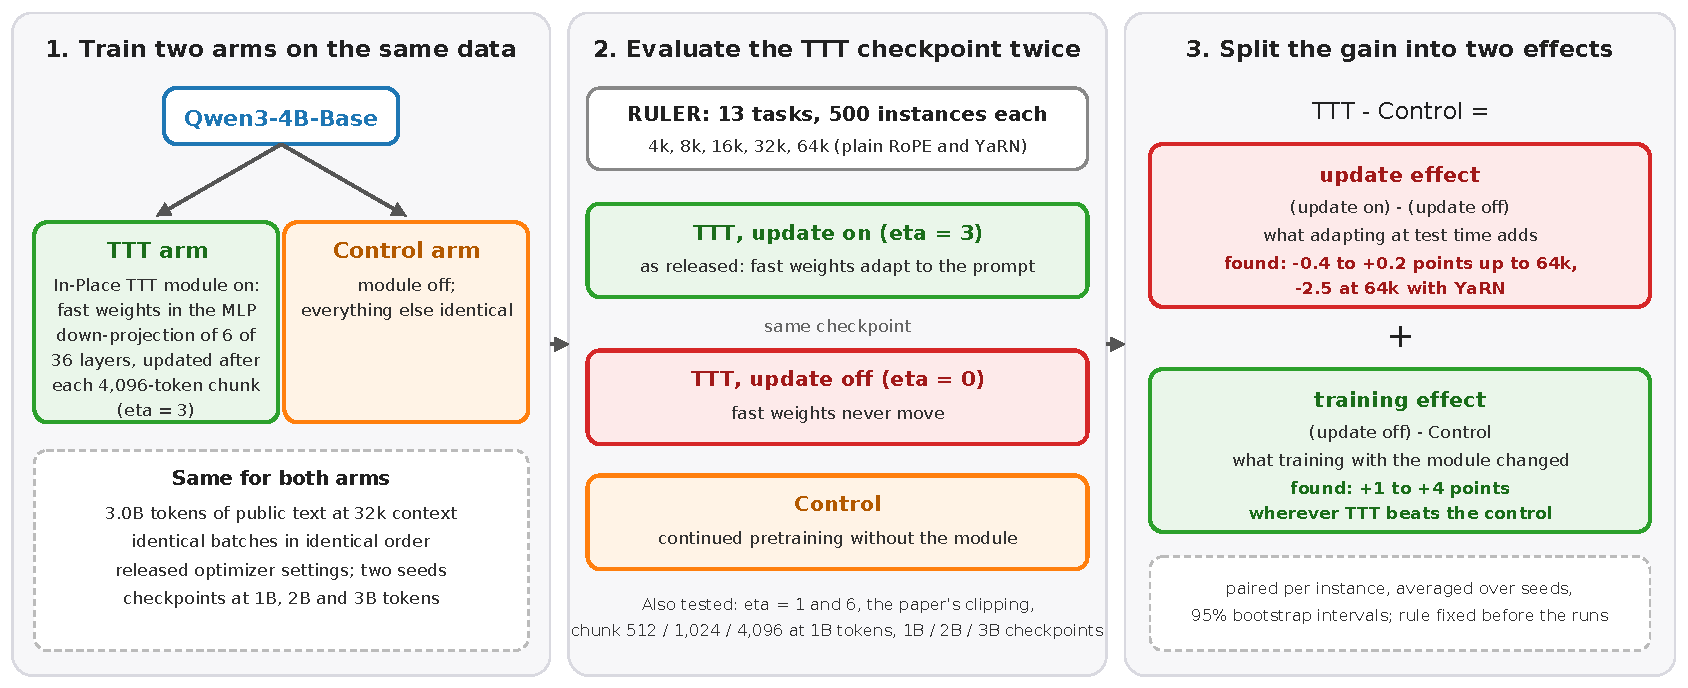
\includegraphics[width=\linewidth]{figures/overview.pdf}
\caption{What was done and tested. Two arms are trained from Qwen3-4B-Base on identical data, with and without the In-Place TTT module (left). The TTT checkpoint is evaluated on RULER twice, with its test-time update on and off, next to the control (middle). The difference between TTT and the control then splits into an update effect and a training effect (right). The update effect is close to zero at all lengths up to 64k with plain RoPE and negative with YaRN; the training effect accounts for the gains.}
\label{fig:overview}
\end{figure}

That comparison leaves the mechanism open. A TTT-trained model differs from its control in two ways. Its shared weights were trained together with a module that changes the inputs of the following layers, and at inference its fast weights adapt to the prompt. The published numbers combine both differences. The method is motivated by the second difference, adaptation at test time, and that difference has not been measured on its own.

The distinction decides how the method should be used. If the update is the source of the gain, longer inputs should help more and the inner learning rate at inference should matter. The update should also transfer beyond the training length. If training with the module is the source, the update is inference overhead that can be switched off, and the training dynamics deserve the attention.

We measure the two effects separately (Figure~\ref{fig:overview}). The same TTT-trained checkpoint is evaluated twice, as released and with the inner learning rate set to zero at inference. The difference between the two evaluations is the effect of the test-time update. The difference between the update-off evaluation and a matched control is the effect of training with the module. We ran this ablation at a reduced budget of 3.0B tokens with two seeds. The arms, the decision rule and the analysis were fixed before the main runs.

Our claim is that at this budget the gain of In-Place TTT on RULER comes from training with the module. Averaged over seeds, the test-time update changes the 13-task mean by between $-0.4$ and $+0.2$ points at lengths up to 64k with plain rotary embeddings. At 64k with YaRN it lowers the mean by 2.5 points. Where the TTT arm beats the control, by 1 to 4 points, the checkpoint with the update disabled shows the same advantage. The study also characterises the recipe. The TTT arm trains with a gradient norm two to four orders of magnitude above the control's, almost all of it in the target convolutions. The released inference code applies no clipping, and the clipping threshold reported for the method removes the update rather than bounding it. The released chunk size of 4,096 is the worst of the three sizes we trained.

\section{Background}

\subsection{In-Place Test-Time Training}

In-Place TTT \citep{feng2026inplace} modifies one layer out of six in the released configuration for Qwen3. In such a layer the MLP down-projection $W \in \mathbb{R}^{d \times d_{\mathrm{ff}}}$ becomes a fast weight. The input is processed in chunks of $c$ tokens, 4,096 in the released configuration. Let $h_t$ be the MLP hidden state at position $t$ and $x_t$ the layer input. The module forms a target per position from a depthwise causal convolution of the layer input, passed through a learned projection $P$. It then updates the down-projection with an outer-product step,
\begin{equation}
W \leftarrow W + \eta \sum_{t=1}^{c} \, (P^{\top} \mathrm{conv}(x)_t)\, h_t^{\top},
\end{equation}
where $\eta$ is the inner learning rate, 3 in the released configuration. The next chunk is read with the updated $W$. The update also runs during training, so the shared weights, the convolution and the projection are trained through it. The convolution is zero-initialised and the projection starts at the identity, so a freshly equipped model computes the same function as the base model.

The release has two properties that matter for this study. The inference code applies the update without normalisation or clipping. The paper's appendix, however, describes rescaling any per-chunk delta whose Frobenius norm exceeds a threshold $\tau$, with $\tau = 10^{-5}$ for Qwen3-4B. We added that rule as an option and tested it. The paper's chunk-size ablation on a 1.7B model also prefers chunks of 512 to 1,024 tokens, while the released configuration uses 4,096. The paper does not state the chunk size or inner learning rate behind its Qwen3-4B results.

\subsection{Related work}

Fast weights written by one network and read by another go back to \citet{ba2016fast}, and \citet{schlag2021linear} showed that linear attention is a fast-weight programmer. Test-time training updates parameters on a self-supervised objective at inference \citep{sun2020ttt}. For language models it has been applied with nearest-neighbour retrieval \citep{hardt2023nearest} and as a recurrent layer whose hidden state is a small model \citep{sun2024ttt}. Titans \citep{behrouz2025titans} learns a memory module with a surprise-based update at test time. In-Place TTT updates existing weights of a pretrained Transformer instead of adding a recurrent block. The same checkpoint can therefore run with or without the update, which is what makes the ablation in this paper possible.

\section{What was tested}

The design was written down before the main runs and is released with the code. Figure~\ref{fig:overview} gives the overview and Table~\ref{tab:arms} lists the arms.

\begin{table}[t]
\caption{Arms. The update-off rows are the TTT checkpoints evaluated with $\eta = 0$, so no separate model is trained. The 1B-token checkpoints of the two main arms (step 477) are the chunk-4,096 and control references for the chunk ablation.}
\label{tab:arms}
\centering
\footnotesize
\resizebox{\textwidth}{!}{\begin{tabular}{llll}
\toprule
Arm & Training & Evaluated as & Seeds \\
\midrule
Base & none & Qwen3-4B-Base as released & -- \\
Control & 3.0B tokens, module disabled & as trained & 1, 2 \\
TTT & 3.0B tokens, released recipe & as trained ($\eta = 3$) & 1, 2 \\
TTT, update off & the TTT checkpoints & $\eta = 0$ & 1, 2 \\
TTT, $\eta$ 1 / 6 / clip & the seed-1 TTT checkpoint & $\eta = 1$; $\eta = 6$; $\eta = 3$ with $\tau = 10^{-5}$ & 1 \\
Chunk 512 / 1,024 & 1.0B tokens, chunk changed & as trained, and with $\eta = 0$ & 1 \\
\bottomrule
\end{tabular}}
\end{table}

\paragraph{Training.} All arms start from Qwen3-4B-Base \citep{yang2025qwen3, qwen3_4b_base}, a 36-layer model with a native context of 32,768 tokens. The TTT arm uses the released recipe. Fast weights are placed in layers 0, 6, 12, 18, 24 and 30, with a learned target projection, a depthwise Conv1D target, $\eta = 3$ and chunk 4,096. The control trains the same model with the module disabled. The rest is identical. Both arms use the released optimizer settings (AdamW, learning rate $5 \times 10^{-6}$ with 2\% warmup and cosine decay, weight decay 0.1, gradient clipping at 1.0). Both use a global batch of 64 sequences of 32,768 tokens for 1,431 steps, which is 3.0B tokens. The seed changes the data order only. A check at the first step hashes the first micro-batch on all ranks, so same-seed arms consume identical batches. The corpus is public. It packs 3.25B tokens into 32,736-token sequences from PG-19 books, arXiv papers, permissively licensed GitHub code and synthetic retrieval documents (Appendix~\ref{app:setup}).

\paragraph{Evaluation.} We use OpenCompass RULER \citep{opencompass2023, hsieh2024ruler}, the framework of the original paper, with its 13 tasks, greedy decoding, 64 generated tokens and base-model prompting. We evaluate 500 instances per task at 4k, 8k, 16k, 32k and 64k. Instances are generated once with a fixed seed, so all arms answer the same prompts and all comparisons are paired. Predictions are re-scored from the saved outputs with RULER's containment rule. Qwen3-4B's native window is 32k. At 64k the primary setting applies YaRN \citep{peng2023yarn} with factor 2 to all arms, as the model card recommends. Plain rotary embeddings \citep{su2021roformer} at 64k are a secondary setting in which all models are beyond their window. At 4k no update fires, because the prompt is shorter than one chunk, so the 4k comparison isolates the training effect by construction.

\paragraph{The ablation.} The update-off variant reproduces the forward pass of the model with the module disabled, with a largest logit difference of 0.0 on held-out text. The active update changes logits by up to 22.7. The attribution at a length is a pair of paired differences. The update effect is TTT minus TTT-update-off. The training effect is TTT-update-off minus control. The two sum to the TTT-minus-control difference. A large update effect would support the stated mechanism. A large training effect would mean that the extra parameters and the training dynamics explain the gain.

\paragraph{Decision rule.} Per arm, seed, length and task we report accuracy with a 95\% bootstrap interval over instances \citep{efron1979bootstrap}. The headline number is the mean over the 13 tasks, as in the original paper. The rule, fixed before the runs, has two conditions. TTT helps at a length if the paired difference TTT minus control, averaged over seeds per instance, has an interval that excludes zero, and if the difference has the same sign in both seeds. The difference between the two seeds of the same arm is reported as the noise floor.

\paragraph{A corpus artifact and the sensitivity analysis.} The synthetic documents end in ``Question: \dots Answer: \dots'' lines after a blank line, which is also the form of RULER's answer prefix. Both trained arms learned to answer two needle tasks, \texttt{niah\_single\_2} and \texttt{niah\_multikey\_1}, by starting a new question block instead of returning the number. The habit is shared by the arms, so paired comparisons stay valid. But the two arms retain it to different degrees at different lengths, and that difference dominates the 13-task means at several lengths. We therefore report all comparisons a second time on the 11 unaffected tasks. This analysis was declared after the seed-1 evaluation and before any seed-2 result; the 13-task analysis stays primary. Appendix~\ref{app:artifact} gives the failure-mode counts.

\section{Results}

\subsection{Does In-Place TTT beat the matched control?}

Table~\ref{tab:means} gives the 13-task means, and Figure~\ref{fig:ruler} plots seed 1. Under the rule, TTT beats the control at 4k, 8k, 16k and 64k with plain RoPE, with seed-averaged margins of 1.1, 1.9, 3.3 and 3.2 points. It does not beat the control at 32k, where seed 1 is 1.8 points behind and seed 2 ties, and the seeds disagree at 64k with YaRN. On the 11 artifact-free tasks the picture is narrower. The two arms are within a point of one another up to 32k in both seeds. TTT leads by 0.6 at 16k and by 3.5 at 64k with plain RoPE, and trails by 2.3 at 64k with YaRN in both seeds (Table~\ref{tab:clean}). The original paper's 32k margin of 0.6 is inside our seed-to-seed spread, which is about a point on the clean tasks at that length.

\begin{table}[t]
\caption{RULER mean over the 13 tasks (500 instances per task; intervals and per-task values in Appendix~\ref{app:pertask}). At 4k no update fires, so the TTT and update-off rows coincide.}
\label{tab:means}
\centering
\small
\begin{tabular}{llrrrrrr}
\toprule
Seed & Arm & 4k & 8k & 16k & 32k & 64k plain & 64k YaRN \\
\midrule
-- & Base & 93.0 & 84.1 & 74.8 & 75.4 & 53.7 & 61.9 \\
\midrule
1 & Control & 85.2 & 82.8 & 78.7 & 77.7 & 47.8 & 64.6 \\
1 & TTT & 86.7 & 84.4 & 82.7 & 75.8 & 50.2 & 59.5 \\
1 & TTT, update off & 86.7 & 84.7 & 83.1 & 75.0 & 51.6 & 63.8 \\
\midrule
2 & Control & 86.5 & 83.5 & 78.8 & 75.5 & 47.8 & 62.6 \\
2 & TTT & 87.3 & 85.8 & 81.4 & 75.5 & 51.7 & 64.2 \\
2 & TTT, update off & 87.3 & 85.8 & 81.9 & 76.0 & 50.2 & 64.9 \\
\bottomrule
\end{tabular}
\end{table}

\begin{figure}[t]
\centering
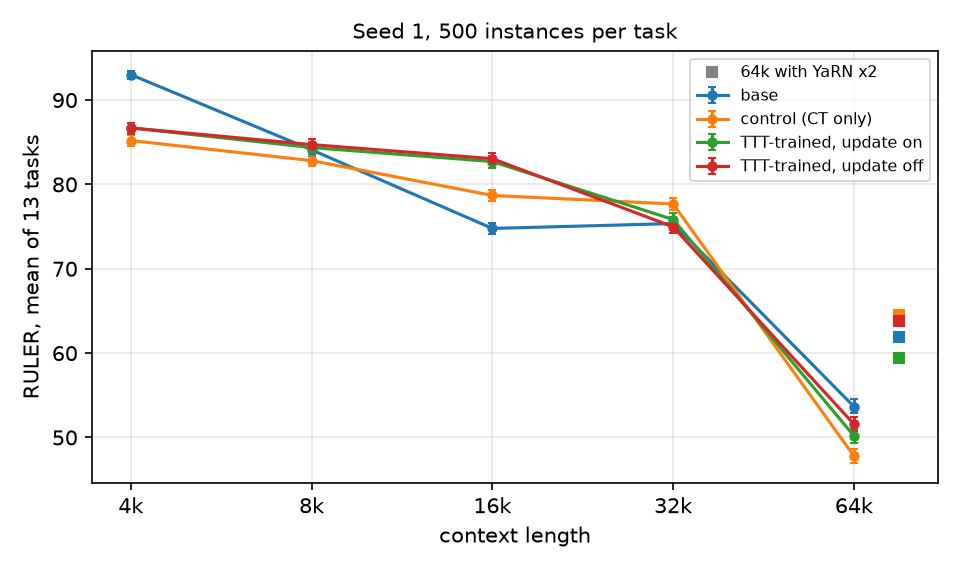
\includegraphics[width=0.78\linewidth]{figures/ruler_seed1.png}
\caption{RULER mean over the 13 tasks by context length for seed 1, with 95\% bootstrap intervals. Squares at the right are the 64k results with YaRN. The TTT checkpoint with the update disabled (red) tracks the same checkpoint with the update active (green) at all lengths. The gap to the control (orange) is the training effect. Seed 2 is in Appendix~\ref{app:figures}.}
\label{fig:ruler}
\end{figure}

\subsection{Is the gain due to the test-time update?}

Figure~\ref{fig:effects} decomposes the TTT-minus-control difference into the update effect and the training effect, per seed and averaged over seeds, and Table~\ref{tab:clean} gives the seed-averaged values on the clean tasks. The update effect is near zero at all lengths up to 64k with plain RoPE. Averaged over seeds it lies between $-0.4$ and $+0.2$ points on the 13 tasks and between $-0.3$ and $+0.4$ on the clean tasks. The training effect accounts for the gains. It is $+1.1$, $+2.1$, $+3.8$ and $+3.1$ points at 4k, 8k, 16k and 64k plain on the 13 tasks, and $+0.9$ and $+3.1$ at 16k and 64k plain on the clean tasks. At 64k with YaRN the update effect is $-2.5$ on the 13 tasks and $-2.6$ on the clean tasks, negative in both seeds. The training effect there is $+0.8$ and $+0.2$. This answers the question. The TTT arm beats the control because its weights were trained differently. Switching the update off at inference has no cost at this budget.

\begin{figure}[t]
\centering
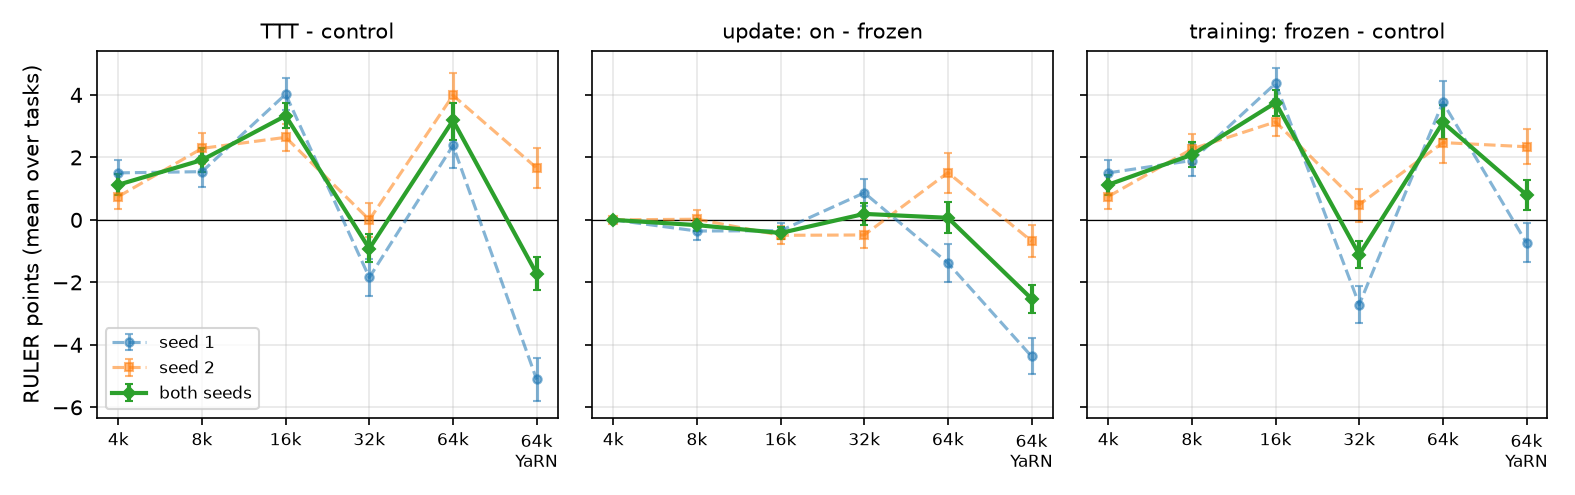
\includegraphics[width=\linewidth]{figures/effects_13.png}
\caption{Paired differences on the same RULER instances, mean over the 13 tasks, with 95\% bootstrap intervals. Left, TTT minus control. Middle, the update effect (TTT minus TTT-update-off). Right, the training effect (TTT-update-off minus control). Dashed lines are single seeds. The solid line averages the two seeds per instance, the estimate the rule uses. The left panel is the sum of the other two. The same figure for the 11 clean tasks is in Appendix~\ref{app:figures}.}
\label{fig:effects}
\end{figure}

\begin{table}[t]
\caption{Seed-averaged paired differences on the 11 tasks without the format artifact (mean over tasks, 95\% bootstrap intervals). ``Rule'' marks settings where the rule is met, with the sign of the verdict. The noise floor is the difference between the two seeds of the TTT arm with the update active / disabled. The 13-task version is Table~\ref{tab:pooled13}.}
\label{tab:clean}
\centering
\footnotesize
\begin{tabular}{lrrrcr}
\toprule
Length & TTT $-$ control & Update effect & Training effect & Rule & Noise floor \\
\midrule
4k & \ci{+0.2}{-0.0}{0.4} & 0.0 & \ci{+0.2}{-0.0}{0.4} & -- & 0.1 / 0.1 \\
8k & \ci{+0.2}{-0.1}{0.4} & \ci{-0.0}{-0.1}{0.1} & \ci{+0.2}{-0.1}{0.4} & -- & 0.1 / 0.1 \\
16k & \ci{+0.6}{0.3}{0.8} & \ci{-0.3}{-0.5}{-0.1} & \ci{+0.9}{0.6}{1.1} & yes ($+$) & 0.3 / 0.1 \\
32k & \ci{-0.2}{-0.5}{0.3} & \ci{-0.0}{-0.4}{0.3} & \ci{-0.1}{-0.5}{0.2} & -- & 1.2 / 0.0 \\
64k plain & \ci{+3.5}{2.8}{4.2} & \ci{+0.4}{-0.2}{0.9} & \ci{+3.1}{2.5}{3.7} & yes ($+$) & 2.3 / 1.4 \\
64k YaRN & \ci{-2.3}{-2.8}{-1.9} & \ci{-2.6}{-3.1}{-2.1} & \ci{+0.2}{-0.1}{0.6} & yes ($-$) & 2.9 / 0.1 \\
\bottomrule
\end{tabular}
\end{table}

The seeds disagree about the update at two settings, and the noise floor locates the disagreement in the update rather than in the weights. At 32k on the clean tasks the update is worth $+0.6$ in seed 1 and $-0.6$ in seed 2, with intervals that exclude zero. At 64k with plain RoPE it is worth $-1.4$ in seed 1 and $+1.5$ in seed 2. The two seeds' TTT arms differ by 1.2 points at 32k with the update active and by 0.0 with it disabled. At 64k with YaRN they differ by 4.8 points with the update active and by 1.1 without it. The trained weights are reproducible across seeds. The behaviour of the update on top of them is not.

\subsection{What does the update do beyond the training length?}

At 64k with YaRN the update harms both seeds, for different reasons. In seed 1 it costs 4.4 points. On the frequent-words task the update-off model lists the three frequent words correctly and scores 93.2. The active update falls into a repetition loop (``1.\ uumoqt - 10 times, 2.\ uumoqt - 9 times, \dots'') and scores 53.7. The released recipe applies no clipping, and after sixteen accumulated chunk updates generation becomes unstable. In seed 2 the update costs 0.7 points and the frequent-words task is unaffected, so the loop belongs to one trained checkpoint. The loss shared by both seeds is on the hardest multi-key needle task. There the update lowers accuracy from 19.0 to 8.0 in seed 1 and from 19.0 to 4.2 in seed 2, by returning another identifier from the haystack or restating the prompt. With plain RoPE at 64k the update's sign depends on the seed. Its seed-2 gain comes from the simplest needle task, where the update-off model answers most failures with a new question block and the update restores the number (36.2 to 63.4). In both seeds two other needle tasks lose 4 to 8 points under the update (Appendix~\ref{app:pertask}).

If the update were the source of the gain, the inner learning rate at inference should matter. Table~\ref{tab:sweep} varies it on the seed-1 checkpoint. At 32k the mean rises by at most 0.9 points at the trained rate and falls at twice that rate. At 64k with plain RoPE any non-zero rate hurts, and the damage grows with the rate. The paper's clipping with $\tau = 10^{-5}$ makes the model indistinguishable from the update-off variant at both lengths. The reason is in the deltas themselves. On held-out 32k text a single chunk changes the down-projection by a Frobenius norm of 0.1 to 0.85. After seven chunks the accumulated change reaches 0.4 to 0.9\% of the weight norm in five of the six TTT layers and 2.3 to 2.4\% in the last. It grows about linearly with no sign of saturation (Appendix~\ref{app:diag}). The threshold is four to five orders of magnitude below those deltas, so a clip at that value removes the update. Within this recipe no inference-time setting makes the update helpful beyond the training length.

\begin{table}[t]
\caption{Inference-time variants of the seed-1 TTT checkpoint, 13-task mean and paired difference to the update-off variant.}
\label{tab:sweep}
\centering
\footnotesize
\begin{tabular}{lrrrr}
\toprule
Variant & 32k & vs.\ update off & 64k plain & vs.\ update off \\
\midrule
$\eta = 0$ (update off) & 75.0 & -- & 51.6 & -- \\
$\eta = 1$ & 75.5 & \ci{+0.5}{0.1}{0.9} & 50.1 & \ci{-1.5}{-2.0}{-1.0} \\
$\eta = 3$ (as trained) & 75.8 & \ci{+0.9}{0.4}{1.3} & 50.2 & \ci{-1.4}{-2.0}{-0.8} \\
$\eta = 6$ & 74.1 & $-0.8$ & 48.2 & $-3.4$ \\
$\eta = 3$, clip $\tau = 10^{-5}$ & 74.8 & \ci{-0.2}{-0.5}{0.2} & 51.7 & \ci{+0.2}{-0.2}{0.5} \\
\bottomrule
\end{tabular}
\end{table}

\subsection{Do the chunk size and the token budget change the picture?}

The chunk size changes how much the active update costs, and the budget changes the sign of the update effect at the training length. Neither changes the conclusion. At 1B tokens the released chunk of 4,096 is the worst of the three sizes with the update active (Table~\ref{tab:chunk}). On the clean tasks chunk 512 beats it by 1.2 points at 32k and by 5.1 at 64k with plain RoPE, and chunk 1,024 by 0.3 and 1.1. This is the direction of the original paper's small-model ablation. The update-off rows show where the 32k ordering comes from. With the update off, the three chunk sizes are within 0.4 points of one another and of the 1B control on the clean tasks. The active update then costs 2.3 points with chunk 4,096, 1.6 with chunk 1,024 and 1.0 with chunk 512. At one third of the budget the chunk size sets how much the update hurts, and training with the module has not changed the shared weights relative to the control. Beyond the window the same split holds with larger numbers. With the update off, the three chunk sizes are within 1.4 points of one another at 64k and lead the 1B control by 7.8 to 9.2 points on the clean tasks. The active update then costs 3.8 points with chunk 4,096, 2.9 with 1,024 and 0.2 with 512. The 64k advantage of the TTT variants over the 1B control is therefore a training effect, and the smaller chunks look better with the update active only because the update hurts them less.

\begin{table}[t]
\caption{Chunk-size ablation at 1.0B tokens (seed-1 recipe, step 477). 13-task means and paired differences to the 1B control on the 11 clean tasks. ``Update off'' rows evaluate the same checkpoint with $\eta = 0$.}
\label{tab:chunk}
\centering
\footnotesize
\begin{tabular}{lrrrr}
\toprule
Model (1B tokens) & 32k & vs.\ control (11) & 64k plain & vs.\ control (11) \\
\midrule
Control & 77.4 & -- & 45.4 & -- \\
Chunk 4,096 (released) & 69.5 & \ci{-2.1}{-2.7}{-1.6} & 49.1 & \ci{+3.9}{3.1}{4.7} \\
Chunk 1,024 & 76.5 & \ci{-1.9}{-2.4}{-1.3} & 50.1 & $+5.0$ \\
Chunk 512 & 73.4 & \ci{-1.0}{-1.5}{-0.4} & 53.5 & $+9.0$ \\
\midrule
Chunk 4,096, update off & 71.3 & \ci{+0.2}{-0.3}{0.6} & 52.7 & \ci{+7.8}{7.1}{8.5} \\
Chunk 1,024, update off & 77.0 & \ci{-0.3}{-0.8}{0.2} & 53.0 & \ci{+8.0}{7.2}{8.7} \\
Chunk 512, update off & 73.8 & \ci{-0.0}{-0.5}{0.5} & 53.9 & \ci{+9.2}{8.4}{9.9} \\
\bottomrule
\end{tabular}
\end{table}

The budget matters up to 2B tokens and not beyond, within the range we trained. Table~\ref{tab:curve} evaluates the seed-1 checkpoints at 1B, 2B and 3B tokens. On the clean tasks at 32k the TTT arm trails the control by 2.1 points at 1B and leads by 0.7 at both 2B and 3B. The update effect in this seed moves from $-2.3$ at 1B to $+0.4$ at 2B and $+0.6$ at 3B, while the training effect stays between $+0.2$ and $+0.3$. The update becomes harmless at the training length as training proceeds; the shared weights do not pull ahead of the control's on the clean tasks at any budget. Beyond the window the picture is stable from 1B tokens on. With plain RoPE at 64k the TTT arm leads the control by 3.7, 4.0 and 2.4 points at 1B, 2B and 3B, and the update-off checkpoint leads by as much or more at all three budgets. The 64k advantage is a training effect throughout, and the update costs 3.8 points at 1B, 0.2 at 2B and 1.5 at 3B on the clean tasks.

\begin{table}[t]
\caption{Learning curve of the seed-1 arms at 32k and at 64k with plain RoPE. 13-task means and paired differences on the 11 clean tasks.}
\label{tab:curve}
\centering
\footnotesize
\resizebox{\textwidth}{!}{\begin{tabular}{llrrrrr}
\toprule
Length & Tokens & Control & TTT & TTT, update off & TTT $-$ control (11) & Update effect (11) \\
\midrule
32k & 1.0B & 77.4 & 69.5 & 71.3 & \ci{-2.1}{-2.7}{-1.6} & \ci{-2.3}{-2.9}{-1.8} \\
32k & 2.0B & 77.9 & 75.6 & 75.1 & \ci{+0.7}{0.2}{1.3} & \ci{+0.4}{0.0}{0.8} \\
32k & 3.0B & 77.7 & 75.8 & 75.0 & \ci{+0.7}{0.2}{1.2} & \ci{+0.6}{0.1}{1.0} \\
\midrule
64k & 1.0B & 45.4 & 49.1 & 52.7 & \ci{+3.9}{3.1}{4.7} & \ci{-3.8}{-4.6}{-3.0} \\
64k & 2.0B & 47.7 & 51.7 & 51.9 & \ci{+4.3}{3.4}{5.1} & \ci{-0.2}{-1.0}{0.5} \\
64k & 3.0B & 47.8 & 50.2 & 51.6 & \ci{+2.3}{1.4}{3.1} & \ci{-1.5}{-2.2}{-0.8} \\
\bottomrule
\end{tabular}}
\end{table}

\subsection{How does the module change training?}

The TTT arm trains in a different regime from the control, which is where its advantage must come from. On identical batches its training loss starts equal to the control's at step 1, because the zero-initialised convolution makes the TTT model equal to the base model. From step 2 on it stays above the control's. The gap shrinks from 0.017 nats over the first 150 steps to 0.007 over the last 143 and does not close within 3B tokens, in both seeds (Table~\ref{tab:phases}). The control's pre-clipping gradient norm stays at 0.2 and is never clipped. The TTT arm's gradient norm starts in the hundreds to thousands and falls to 20 to 30. The released clipping at 1.0 therefore rescales the whole network's gradient at all steps, by a factor of about 50 near the end. On held-out text the final TTT checkpoints have a gradient norm of 49.6 and 49.2 (seeds 1 and 2). Of this, 49.6 and 49.2 lie in the six target convolutions, which hold 76,800 of the model's 4.0B parameters. The base model with a freshly initialised module already has a convolution gradient 14 times the rest of the network's, so the imbalance exists from the first step. On eight held-out 16k sequences the controls reach 1.823 and 1.822 nats, the TTT arms 1.832 and 1.831, and the base model 1.865. The loss penalty therefore persists outside the training data. At inference the module is cheap. Prefill plus 64 generated tokens at batch size 1 takes at most 2\% longer than without the module, and peak memory is 0.38 GB higher (Appendix~\ref{app:diag}).

\section{Discussion}

The ablation answers the question the published evaluation leaves open. At a 3B-token budget the advantage of an In-Place TTT model over a matched control is present when the fast weights never move. The update is close to neutral at and below the training length and harmful beyond it under the recommended positional scaling. The TTT model is better than the control because it was trained differently.

The training data suggest how. The gradient that reaches the shared weights is rescaled at all steps by a norm that lives in 76,800 convolution parameters. The training loss stays 0.007 nats higher on identical batches. The chunk size does not change the function the update-off model computes, yet it moves RULER by several points. The module therefore acts as a regulariser and an optimiser perturbation during training. Whether a cheaper perturbation, for example the same gradient rescaling without the module, would produce the same training effect is a question this study was not designed to answer.

Our results reinterpret the original paper's numbers rather than contradict them. That paper reports $+0.6$ at 32k and $+4.4$ at 64k at roughly ten times our budget and with a 64k training stage we did not run. An effect of 0.6 points at 32k is inside our noise floor. At 64k with YaRN we find the opposite sign and a cause, the unclipped update. The paper describes clipping at $\tau = 10^{-5}$, and on our checkpoints that value switches the update off. Either the paper's models produce deltas five orders of magnitude smaller than ours, or its 64k gains came from models whose update was disabled in effect at inference. The released code and configuration do not let us tell which.

\paragraph{Limitations.} Our budget is 3.0B tokens per arm at 32k, against the paper's 20B at 32k followed by 15B at 64k. Our 64k numbers therefore test extrapolation beyond the training length, and effects that need more tokens would be missed. The corpus differs from the paper's, and its synthetic documents introduced the format artifact, which we handle with a sensitivity analysis declared after the seed-1 results. We studied one model, one benchmark with greedy decoding, and two seeds. The learning-rate sweep, the clipping test and the learning curve use seed 1 only, the chunk ablation stops at 1B tokens, and one clipping threshold was tested. Bootstrap intervals cover instance sampling only, and the noise floor shows that single-seed differences of a point or less should be read with care. The upstream code is pinned, with small patches that add configuration validation, metrics logging and the optional clipping. Any difference between the released code and the code behind the paper therefore affects these results as well.

\section{Conclusion}

An In-Place TTT model differs from its control in two ways, training with the module and adapting at test time. We separated them by evaluating the same checkpoints with the update switched off. At a 3B-token budget on Qwen3-4B, the RULER gains over the matched control come from training with the module. The test-time update contributes at most 0.4 points on average at lengths up to 64k and changes sign between seeds where it is not zero. At 64k with YaRN it costs 2.5 points. This matters for practice because the update can be switched off at inference without loss at this budget. It matters for the method because the training dynamics, rather than the update rule, are where the gain comes from. The recipe trains in a gradient regime set by its target convolutions, pays a persistent loss penalty and uses the worst of three chunk sizes. It applies no clipping at inference, while the threshold reported for it removes the update. A rule that bounds the update without removing it is needed before the update can be trusted beyond the training length. Whether larger budgets or a 64k training stage change the balance is the natural next experiment. The released code runs it from one configuration file.

\subsubsection*{Reproducibility statement}

We release the code, the training and evaluation configurations, and the three patches on the pinned upstream commit. We also release the corpus builder with pinned dataset revisions, the study plan, all per-instance predictions, and the analysis scripts that regenerate the tables and figures of this paper. Paths in the repository are relative, and numbers in the results log name the job and run directory they came from.

\bibliography{refs}
\bibliographystyle{iclr2026_conference}

\clearpage
\appendix

\section{Training, data and evaluation details}\label{app:setup}

\paragraph{Training.} VeOmni \citep{ma2025veomni} at the commit pinned by the released In-Place TTT code \citep{inplacettt_code}, with FSDP2 \citep{zhao2023fsdp}, FlashAttention-2 \citep{dao2023flashattention2}, Liger kernels \citep{hsu2024liger}, bf16 compute with fp32 master weights, gradient checkpointing and micro-batch 2. Checkpoints were saved at steps 477, 954 and 1,431 (1B, 2B and 3B tokens). Table~\ref{tab:hparams} lists the configuration.

\begin{table}[H]
\caption{Training configuration (identical for both arms except \texttt{ttt\_mode}).}
\label{tab:hparams}
\centering
\footnotesize
\resizebox{\textwidth}{!}{\begin{tabular}{ll}
\toprule
Model & Qwen3-4B-Base (36 layers, hidden 2,560, MLP 9,728) \\
TTT layers & 0, 6, 12, 18, 24, 30 \\
Target & depthwise Conv1D, zero-initialised; learned projection, identity-initialised \\
Inner learning rate $\eta$ & 3 \\
Chunk & 4,096 (512 and 1,024 in the ablation) \\
Sequence length & 32,768 \\
Global batch & 64 sequences (2.1M tokens) \\
Steps & 1,431 (3.0B tokens) \\
Optimizer & AdamW, lr $5 \times 10^{-6}$, 2\% warmup, cosine decay, weight decay 0.1 \\
Gradient clipping & 1.0 \\
Seeds & 1, 2 (data order) \\
\bottomrule
\end{tabular}}
\end{table}

\paragraph{Corpus.} Table~\ref{tab:corpus} lists the sources. Documents longer than one sequence continue into the next, sequences are shuffled globally with a fixed seed, and a manifest records dataset revisions and counts. All sequences re-tokenise to between 32,704 and 32,737 tokens. The 1,431 steps consume 91,584 of the 99,217 sequences, and 64 sequences are held out for loss checks. The synthetic documents are of two kinds, mixed equally. One is a key-value table of 8-character keys and 6-digit values followed by four ``Question: What is the value of key \dots? Answer: \dots'' lines. The other is a book passage with three to eight planted sentences of the form ``The access code for the $\langle$object$\rangle$ in $\langle$city$\rangle$ is $\langle$code$\rangle$.'' followed by a question about them. The question line after a blank line is what the trained models reproduce on RULER.

\begin{table}[H]
\caption{Training corpus (3.25B tokens in 99,217 sequences of 32,736 tokens).}
\label{tab:corpus}
\centering
\footnotesize
\resizebox{\textwidth}{!}{\begin{tabular}{llrr}
\toprule
Source & Dataset & Sequences & Tokens \\
\midrule
Books & \texttt{emozilla/pg19} \citep{rae2019compressive, pg19_hf} & 39,712 & 1.30B \\
Papers & \texttt{ccdv/arxiv-summarization} \citep{cohan2018discourse, arxiv_summarization_hf} & 22,911 & 0.75B \\
Code & \texttt{codeparrot/github-code-clean} \citep{codeparrot_github_code_clean} (permissive licenses, by repository) & 27,493 & 0.90B \\
Synthetic & key-value and planted-fact retrieval documents & 9,165 & 0.30B \\
\bottomrule
\end{tabular}}
\end{table}

\paragraph{Evaluation.} OpenCompass 0.5.4 with the RULER configuration it ships, batch size 1 (the released inference code applies the fast-weight update only to the first sequence of a batch), and the TTT inference classes registered in all workers. Variants ($\eta$ 0, 1, 6; clipping; YaRN factor 2) are symlinked copies of a checkpoint with an edited configuration file. A calibration run of the base model with 100 instances per task gave a 4k mean of 93.5, against 96.6 reported by the original paper for its continually trained baseline. Task means re-scored from the saved outputs agree with OpenCompass's own.

\section{The format artifact}\label{app:artifact}

Wrong answers were classified into three modes, a new ``Question:'' block, an empty answer, or other. Table~\ref{tab:failure} gives the share of new-question answers on the two affected tasks. At 4k both trained arms fail on \texttt{niah\_single\_2} in this way about two thirds of the time in seed 1 and half the time in seed 2. At 32k the seed-1 control had almost stopped, while the seed-1 TTT weights continued with or without the update, which is the whole 32k deficit of that seed on the 13 tasks. In seed 2 both arms continued at similar rates and tie at 32k.

\begin{table}[H]
\caption{Share of answers (\%) that start a new ``Question:'' block, by arm and length, on the two tasks affected by the corpus artifact.}
\label{tab:failure}
\centering
\footnotesize
\begin{tabular}{llrrrr}
\toprule
Task & Length & Base & Control & TTT & TTT, update off \\
\midrule
NIAH single 2 & 4k, seed 1 & 0 & 65 & 64 & 64 \\
NIAH single 2 & 4k, seed 2 & 0 & 50 & 59 & 59 \\
NIAH single 2 & 32k, seed 1 & 0 & 1 & 36 & 41 \\
NIAH single 2 & 32k, seed 2 & 0 & 31 & 36 & 36 \\
NIAH single 2 & 64k YaRN, seed 1 & 0 & 3 & 63 & 54 \\
NIAH single 2 & 64k YaRN, seed 2 & 0 & 33 & 39 & 40 \\
NIAH multikey 1 & 32k, seed 1 & 0 & 41 & 61 & 61 \\
NIAH multikey 1 & 32k, seed 2 & 0 & 45 & 47 & 49 \\
\bottomrule
\end{tabular}
\end{table}

\section{Seed-averaged differences on the 13 tasks}\label{app:pooled}

\begin{table}[H]
\caption{Seed-averaged paired differences on the 13 tasks (companion to Table~\ref{tab:clean}).}
\label{tab:pooled13}
\centering
\footnotesize
\begin{tabular}{lrrrcr}
\toprule
Length & TTT $-$ control & Update effect & Training effect & Rule & Noise floor \\
\midrule
4k & \ci{+1.1}{0.8}{1.5} & 0.0 & \ci{+1.1}{0.8}{1.4} & yes ($+$) & 0.5 / 0.5 \\
8k & \ci{+1.9}{1.5}{2.3} & \ci{-0.2}{-0.4}{0.0} & \ci{+2.1}{1.7}{2.5} & yes ($+$) & 1.5 / 1.1 \\
16k & \ci{+3.3}{2.9}{3.8} & \ci{-0.4}{-0.6}{-0.2} & \ci{+3.8}{3.3}{4.2} & yes ($+$) & 1.3 / 1.1 \\
32k & \ci{-0.9}{-1.4}{-0.5} & \ci{+0.2}{-0.1}{0.5} & \ci{-1.1}{-1.5}{-0.7} & no & 0.3 / 1.0 \\
64k plain & \ci{+3.2}{2.6}{3.8} & \ci{+0.1}{-0.4}{0.6} & \ci{+3.1}{2.5}{3.7} & yes ($+$) & 1.5 / 1.4 \\
64k YaRN & \ci{-1.7}{-2.3}{-1.2} & \ci{-2.5}{-3.0}{-2.1} & \ci{+0.8}{0.3}{1.3} & no & 4.8 / 1.1 \\
\bottomrule
\end{tabular}
\end{table}

Per-seed values on the 13 tasks, TTT minus control at 4k / 8k / 16k / 32k / 64k plain / 64k YaRN, are $+1.5$ / $+1.5$ / $+4.0$ / $-1.8$ / $+2.4$ / $-5.1$ for seed 1 and $+0.7$ / $+2.3$ / $+2.6$ / $0.0$ / $+4.0$ / $+1.7$ for seed 2. The update effects are $0.0$ / $-0.4$ / $-0.3$ / $+0.9$ / $-1.4$ / $-4.4$ and $0.0$ / $0.0$ / $-0.5$ / $-0.5$ / $+1.5$ / $-0.7$.

\section{Per-task results}\label{app:pertask}

Tables~\ref{tab:pt4k} to \ref{tab:pt64ky} give per-task accuracies for both seeds at all lengths. The mean row carries the 95\% bootstrap interval. NIAH tasks are needle-in-a-haystack variants.

\begin{table}[H]\caption{Per-task accuracy at 4k.}\label{tab:pt4k}\centering\resizebox{\textwidth}{!}{\begin{tabular}{lrrrrrrr}
\toprule
Task & Base & Control~s1 & TTT~s1 & TTT~s1~frozen & Control~s2 & TTT~s2 & TTT~s2~frozen \\
\midrule
NIAH single 1 & 100.0 & 99.8 & 99.8 & 99.8 & 100.0 & 99.2 & 99.2 \\
NIAH single 2 & 100.0 & 35.4 & 36.0 & 36.0 & 50.4 & 40.8 & 40.8 \\
NIAH single 3 & 100.0 & 98.8 & 98.4 & 98.4 & 99.0 & 99.0 & 99.0 \\
NIAH multikey 1 & 93.8 & 64.6 & 82.0 & 82.0 & 65.6 & 82.8 & 82.8 \\
NIAH multikey 2 & 99.0 & 98.8 & 99.4 & 99.4 & 99.0 & 99.2 & 99.2 \\
NIAH multikey 3 & 99.6 & 99.8 & 99.6 & 99.6 & 99.8 & 99.8 & 99.8 \\
NIAH multiquery & 99.3 & 98.2 & 98.7 & 98.7 & 98.6 & 99.2 & 99.2 \\
NIAH multivalue & 99.1 & 99.8 & 99.8 & 99.8 & 99.7 & 99.8 & 99.8 \\
Variable tracking & 100.0 & 100.0 & 100.0 & 100.0 & 100.0 & 100.0 & 100.0 \\
Common words & 93.9 & 96.2 & 96.4 & 96.4 & 95.2 & 96.1 & 96.1 \\
Frequent words & 90.3 & 89.8 & 89.1 & 89.1 & 90.1 & 89.9 & 89.9 \\
QA SQuAD & 80.0 & 76.8 & 77.2 & 77.2 & 77.4 & 78.6 & 78.6 \\
QA HotpotQA & 54.2 & 49.6 & 50.8 & 50.8 & 49.8 & 50.0 & 50.0 \\
\midrule
Mean & 93.0 [92.5, 93.5] & 85.2 [84.6, 85.8] & 86.7 [86.1, 87.3] & 86.7 [86.1, 87.3] & 86.5 [85.8, 87.2] & 87.3 [86.6, 87.9] & 87.3 [86.6, 87.9] \\
\bottomrule
\end{tabular}
}\end{table}
\begin{table}[H]\caption{Per-task accuracy at 8k.}\label{tab:pt8k}\centering\resizebox{\textwidth}{!}{\begin{tabular}{lrrrrrrr}
\toprule
Task & Base & Control~s1 & TTT~s1 & TTT~s1~frozen & Control~s2 & TTT~s2 & TTT~s2~frozen \\
\midrule
NIAH single 1 & 100.0 & 99.0 & 99.6 & 99.8 & 100.0 & 97.8 & 98.8 \\
NIAH single 2 & 65.2 & 63.6 & 65.0 & 68.4 & 72.6 & 76.2 & 76.4 \\
NIAH single 3 & 99.0 & 97.6 & 98.8 & 98.8 & 97.2 & 98.6 & 98.6 \\
NIAH multikey 1 & 49.6 & 29.6 & 44.8 & 46.2 & 28.2 & 54.2 & 53.2 \\
NIAH multikey 2 & 96.8 & 98.2 & 98.8 & 99.0 & 98.6 & 98.6 & 98.8 \\
NIAH multikey 3 & 95.4 & 95.2 & 96.4 & 96.4 & 95.0 & 95.8 & 96.0 \\
NIAH multiquery & 97.0 & 99.0 & 98.9 & 98.8 & 99.1 & 98.8 & 98.8 \\
NIAH multivalue & 97.1 & 99.0 & 98.6 & 98.7 & 99.0 & 98.5 & 98.4 \\
Variable tracking & 99.9 & 100.0 & 100.0 & 99.9 & 99.9 & 99.9 & 99.9 \\
Common words & 81.3 & 87.0 & 87.0 & 87.1 & 88.7 & 89.1 & 88.3 \\
Frequent words & 95.3 & 95.9 & 95.3 & 95.5 & 95.7 & 95.1 & 95.0 \\
QA SQuAD & 66.2 & 65.8 & 66.4 & 65.8 & 66.4 & 66.0 & 66.4 \\
QA HotpotQA & 50.4 & 46.8 & 47.2 & 47.0 & 45.8 & 47.2 & 47.0 \\
\midrule
Mean & 84.1 [83.4, 84.8] & 82.8 [82.1, 83.5] & 84.4 [83.7, 85.1] & 84.7 [84.0, 85.4] & 83.5 [82.9, 84.2] & 85.8 [85.1, 86.5] & 85.8 [85.2, 86.5] \\
\bottomrule
\end{tabular}
}\end{table}
\begin{table}[H]\caption{Per-task accuracy at 16k.}\label{tab:pt16k}\centering\resizebox{\textwidth}{!}{\begin{tabular}{lrrrrrrr}
\toprule
Task & Base & Control~s1 & TTT~s1 & TTT~s1~frozen & Control~s2 & TTT~s2 & TTT~s2~frozen \\
\midrule
NIAH single 1 & 100.0 & 100.0 & 100.0 & 100.0 & 100.0 & 100.0 & 100.0 \\
NIAH single 2 & 20.2 & 61.4 & 86.0 & 89.0 & 61.8 & 79.4 & 79.6 \\
NIAH single 3 & 94.4 & 94.2 & 97.8 & 98.2 & 93.6 & 96.4 & 97.4 \\
NIAH multikey 1 & 8.2 & 8.6 & 28.2 & 28.6 & 9.4 & 21.8 & 22.4 \\
NIAH multikey 2 & 96.2 & 97.4 & 98.0 & 97.6 & 98.2 & 98.0 & 97.4 \\
NIAH multikey 3 & 85.4 & 88.8 & 90.4 & 92.2 & 89.2 & 87.2 & 91.0 \\
NIAH multiquery & 96.1 & 98.2 & 98.2 & 98.0 & 98.0 & 97.8 & 98.0 \\
NIAH multivalue & 98.2 & 99.3 & 99.1 & 99.2 & 99.3 & 99.2 & 99.2 \\
Variable tracking & 99.9 & 99.9 & 100.0 & 100.0 & 99.9 & 99.9 & 99.9 \\
Common words & 65.8 & 71.4 & 72.8 & 72.0 & 71.3 & 73.7 & 72.7 \\
Frequent words & 98.3 & 97.1 & 97.8 & 98.0 & 97.7 & 97.8 & 97.9 \\
QA SQuAD & 65.0 & 63.4 & 63.6 & 63.2 & 63.6 & 64.0 & 64.8 \\
QA HotpotQA & 44.4 & 43.2 & 43.4 & 43.8 & 42.2 & 43.6 & 44.8 \\
\midrule
Mean & 74.8 [74.1, 75.4] & 78.7 [78.0, 79.4] & 82.7 [82.0, 83.4] & 83.1 [82.4, 83.7] & 78.8 [78.1, 79.5] & 81.4 [80.8, 82.1] & 81.9 [81.3, 82.6] \\
\bottomrule
\end{tabular}
}\end{table}
\begin{table}[H]\caption{Per-task accuracy at 32k.}\label{tab:pt32k}\centering\resizebox{\textwidth}{!}{\begin{tabular}{lrrrrrrr}
\toprule
Task & Base & Control~s1 & TTT~s1 & TTT~s1~frozen & Control~s2 & TTT~s2 & TTT~s2~frozen \\
\midrule
NIAH single 1 & 100.0 & 99.2 & 100.0 & 100.0 & 100.0 & 99.8 & 100.0 \\
NIAH single 2 & 83.2 & 98.4 & 63.6 & 58.6 & 68.8 & 63.8 & 63.6 \\
NIAH single 3 & 97.6 & 97.6 & 98.4 & 98.2 & 97.4 & 97.4 & 97.4 \\
NIAH multikey 1 & 45.2 & 27.0 & 30.0 & 29.8 & 22.0 & 38.2 & 38.2 \\
NIAH multikey 2 & 84.8 & 88.2 & 91.6 & 89.2 & 91.2 & 90.0 & 88.4 \\
NIAH multikey 3 & 46.0 & 69.2 & 75.8 & 75.0 & 72.8 & 65.2 & 72.6 \\
NIAH multiquery & 94.5 & 94.7 & 95.9 & 95.0 & 94.7 & 95.3 & 95.5 \\
NIAH multivalue & 96.1 & 98.0 & 98.0 & 98.0 & 98.2 & 98.0 & 98.2 \\
Variable tracking & 99.7 & 99.6 & 99.7 & 99.7 & 99.6 & 99.5 & 99.5 \\
Common words & 47.1 & 53.1 & 52.3 & 50.1 & 51.8 & 52.5 & 51.6 \\
Frequent words & 96.0 & 95.0 & 95.3 & 95.3 & 95.3 & 95.8 & 95.8 \\
QA SQuAD & 51.2 & 51.4 & 47.8 & 48.8 & 50.8 & 48.0 & 49.0 \\
QA HotpotQA & 38.2 & 38.4 & 37.6 & 37.0 & 38.8 & 38.0 & 37.8 \\
\midrule
Mean & 75.4 [74.6, 76.2] & 77.7 [77.0, 78.4] & 75.8 [75.1, 76.6] & 75.0 [74.2, 75.7] & 75.5 [74.8, 76.2] & 75.5 [74.7, 76.3] & 76.0 [75.2, 76.8] \\
\bottomrule
\end{tabular}
}\end{table}
\begin{table}[H]\caption{Per-task accuracy at 64k with plain RoPE.}\label{tab:pt64k}\centering\resizebox{\textwidth}{!}{\begin{tabular}{lrrrrrrr}
\toprule
Task & Base & Control~s1 & TTT~s1 & TTT~s1~frozen & Control~s2 & TTT~s2 & TTT~s2~frozen \\
\midrule
NIAH single 1 & 86.8 & 45.8 & 51.2 & 46.4 & 34.2 & 63.4 & 36.2 \\
NIAH single 2 & 83.4 & 82.8 & 85.6 & 85.0 & 84.4 & 82.8 & 83.8 \\
NIAH single 3 & 95.8 & 71.2 & 83.8 & 88.6 & 71.4 & 79.4 & 83.4 \\
NIAH multikey 1 & 52.4 & 50.6 & 54.0 & 56.0 & 50.4 & 51.6 & 55.4 \\
NIAH multikey 2 & 25.2 & 9.0 & 18.4 & 23.6 & 18.2 & 15.6 & 23.4 \\
NIAH multikey 3 & 2.2 & 2.6 & 1.6 & 3.2 & 2.2 & 0.6 & 2.6 \\
NIAH multiquery & 53.5 & 61.9 & 64.7 & 63.6 & 60.4 & 64.8 & 63.4 \\
NIAH multivalue & 62.6 & 73.7 & 74.8 & 75.6 & 74.8 & 76.0 & 75.7 \\
Variable tracking & 95.3 & 94.8 & 96.3 & 95.2 & 95.7 & 96.8 & 96.0 \\
Common words & 11.7 & 16.9 & 18.3 & 16.3 & 16.0 & 19.2 & 16.8 \\
Frequent words & 81.3 & 70.7 & 59.3 & 73.5 & 72.5 & 81.2 & 73.7 \\
QA SQuAD & 27.6 & 24.6 & 25.0 & 24.6 & 23.6 & 22.4 & 23.8 \\
QA HotpotQA & 19.8 & 17.2 & 19.6 & 18.8 & 17.0 & 18.8 & 18.8 \\
\midrule
Mean & 53.7 [52.8, 54.5] & 47.8 [47.0, 48.7] & 50.2 [49.4, 51.0] & 51.6 [50.8, 52.4] & 47.8 [46.9, 48.6] & 51.7 [50.9, 52.5] & 50.2 [49.4, 51.1] \\
\bottomrule
\end{tabular}
}\end{table}
\begin{table}[H]\caption{Per-task accuracy at 64k with YaRN $\times 2$.}\label{tab:pt64ky}\centering\resizebox{\textwidth}{!}{\begin{tabular}{lrrrrrrr}
\toprule
Task & Base & Control~s1 & TTT~s1 & TTT~s1~frozen & Control~s2 & TTT~s2 & TTT~s2~frozen \\
\midrule
NIAH single 1 & 99.4 & 98.4 & 99.6 & 98.2 & 92.6 & 100.0 & 98.8 \\
NIAH single 2 & 70.0 & 73.0 & 32.4 & 38.8 & 43.6 & 54.4 & 52.6 \\
NIAH single 3 & 96.0 & 96.4 & 97.2 & 97.6 & 96.2 & 96.6 & 97.6 \\
NIAH multikey 1 & 26.6 & 11.8 & 28.2 & 33.4 & 15.8 & 35.8 & 34.8 \\
NIAH multikey 2 & 58.6 & 72.4 & 76.0 & 70.0 & 77.6 & 72.2 & 69.2 \\
NIAH multikey 3 & 12.4 & 13.2 & 8.0 & 19.0 & 14.8 & 4.2 & 19.0 \\
NIAH multiquery & 80.6 & 87.9 & 90.5 & 89.0 & 88.5 & 89.5 & 89.1 \\
NIAH multivalue & 88.4 & 94.3 & 95.4 & 95.0 & 94.3 & 94.9 & 94.3 \\
Variable tracking & 99.0 & 98.5 & 98.1 & 98.9 & 98.8 & 98.8 & 99.1 \\
Common words & 13.8 & 30.9 & 25.6 & 27.4 & 30.5 & 27.4 & 27.4 \\
Frequent words & 93.9 & 92.9 & 53.7 & 93.2 & 93.1 & 93.5 & 93.1 \\
QA SQuAD & 38.0 & 43.4 & 43.2 & 43.8 & 42.4 & 42.4 & 42.8 \\
QA HotpotQA & 27.6 & 26.2 & 25.0 & 25.4 & 25.0 & 25.2 & 25.8 \\
\midrule
Mean & 61.9 [61.1, 62.7] & 64.6 [63.8, 65.3] & 59.5 [58.7, 60.2] & 63.8 [63.0, 64.6] & 62.6 [61.8, 63.3] & 64.2 [63.5, 65.0] & 64.9 [64.1, 65.7] \\
\bottomrule
\end{tabular}
}\end{table}

\section{Sweep, chunk and learning-curve tables}\label{app:sweep}

\begin{table}[H]\caption{Per-task accuracy of the inference-time variants (seed 1) at 32k.}\centering\resizebox{\textwidth}{!}{\begin{tabular}{lrrrrr}
\toprule
Task & lr~0 & lr~1 & lr~3 & lr~6 & lr~3,~clip \\
\midrule
NIAH single 1 & 100.0 & 100.0 & 100.0 & 92.2 & 100.0 \\
NIAH single 2 & 58.6 & 61.4 & 63.6 & 72.2 & 57.6 \\
NIAH single 3 & 98.2 & 98.0 & 98.4 & 98.2 & 98.4 \\
NIAH multikey 1 & 29.8 & 30.6 & 30.0 & 31.6 & 29.6 \\
NIAH multikey 2 & 89.2 & 89.6 & 91.6 & 92.0 & 88.6 \\
NIAH multikey 3 & 75.0 & 74.8 & 75.8 & 67.2 & 75.2 \\
NIAH multiquery & 95.0 & 95.2 & 95.9 & 95.5 & 95.3 \\
NIAH multivalue & 98.0 & 98.0 & 98.0 & 98.3 & 98.0 \\
Variable tracking & 99.7 & 99.6 & 99.7 & 99.6 & 99.7 \\
Common words & 50.1 & 50.9 & 52.3 & 51.1 & 49.9 \\
Frequent words & 95.3 & 95.6 & 95.3 & 79.1 & 95.5 \\
QA SQuAD & 48.8 & 49.6 & 47.8 & 48.4 & 48.4 \\
QA HotpotQA & 37.0 & 37.8 & 37.6 & 38.4 & 36.6 \\
\midrule
Mean & 75.0 [74.2, 75.8] & 75.5 [74.7, 76.3] & 75.8 [75.1, 76.6] & 74.1 [73.4, 74.9] & 74.8 [74.0, 75.6] \\
\bottomrule
\end{tabular}
}\end{table}
\begin{table}[H]\caption{Per-task accuracy of the inference-time variants (seed 1) at 64k, plain RoPE.}\centering\resizebox{\textwidth}{!}{\begin{tabular}{lrrrrr}
\toprule
Task & lr~0 & lr~1 & lr~3 & lr~6 & lr~3,~clip \\
\midrule
NIAH single 1 & 46.4 & 37.0 & 51.2 & 99.4 & 47.6 \\
NIAH single 2 & 85.0 & 85.0 & 85.6 & 84.0 & 85.6 \\
NIAH single 3 & 88.6 & 86.8 & 83.8 & 79.4 & 90.4 \\
NIAH multikey 1 & 56.0 & 56.0 & 54.0 & 52.4 & 55.4 \\
NIAH multikey 2 & 23.6 & 24.0 & 18.4 & 20.2 & 22.8 \\
NIAH multikey 3 & 3.2 & 2.4 & 1.6 & 0.4 & 3.4 \\
NIAH multiquery & 63.6 & 64.2 & 64.7 & 66.2 & 63.4 \\
NIAH multivalue & 75.6 & 76.0 & 74.8 & 75.4 & 75.7 \\
Variable tracking & 95.2 & 95.5 & 96.3 & 92.3 & 95.0 \\
Common words & 16.3 & 17.2 & 18.3 & 9.1 & 16.3 \\
Frequent words & 73.5 & 63.7 & 59.3 & 2.7 & 73.3 \\
QA SQuAD & 24.6 & 24.6 & 25.0 & 25.4 & 24.6 \\
QA HotpotQA & 18.8 & 18.6 & 19.6 & 19.6 & 19.0 \\
\midrule
Mean & 51.6 [50.8, 52.4] & 50.1 [49.3, 51.0] & 50.2 [49.4, 51.0] & 48.2 [47.5, 48.9] & 51.7 [50.9, 52.6] \\
\bottomrule
\end{tabular}
}\end{table}
\begin{table}[H]\caption{Per-task accuracy of the 1B-token chunk-size models at 32k.}\centering\resizebox{\textwidth}{!}{\begin{tabular}{lrrrrrrr}
\toprule
Task & Control~1B & Chunk~4096 & 4096~frozen & Chunk~1024 & 1024~frozen & Chunk~512 & 512~frozen \\
\midrule
NIAH single 1 & 99.0 & 98.4 & 99.8 & 99.8 & 100.0 & 97.6 & 99.4 \\
NIAH single 2 & 99.2 & 29.2 & 29.8 & 93.4 & 84.8 & 57.2 & 48.2 \\
NIAH single 3 & 97.8 & 96.6 & 97.0 & 97.4 & 97.0 & 96.6 & 97.4 \\
NIAH multikey 1 & 30.0 & 22.0 & 18.6 & 45.2 & 42.8 & 31.8 & 34.8 \\
NIAH multikey 2 & 88.2 & 88.8 & 88.8 & 87.8 & 86.6 & 91.0 & 88.0 \\
NIAH multikey 3 & 66.2 & 51.2 & 69.0 & 54.8 & 67.0 & 59.8 & 69.4 \\
NIAH multiquery & 94.6 & 94.8 & 95.2 & 95.6 & 95.5 & 95.0 & 94.8 \\
NIAH multivalue & 97.8 & 98.2 & 98.5 & 97.9 & 97.8 & 97.7 & 97.8 \\
Variable tracking & 99.8 & 99.8 & 99.5 & 99.7 & 99.6 & 99.6 & 99.6 \\
Common words & 48.7 & 44.4 & 48.2 & 43.7 & 47.9 & 48.2 & 49.5 \\
Frequent words & 94.9 & 94.4 & 95.2 & 93.2 & 95.3 & 94.1 & 95.3 \\
QA SQuAD & 50.0 & 48.2 & 48.2 & 48.2 & 49.2 & 48.8 & 47.6 \\
QA HotpotQA & 39.6 & 38.0 & 39.0 & 38.0 & 37.4 & 37.4 & 37.6 \\
\midrule
Mean & 77.4 [76.6, 78.1] & 69.5 [68.8, 70.4] & 71.3 [70.5, 72.0] & 76.5 [75.7, 77.3] & 77.0 [76.2, 77.8] & 73.4 [72.6, 74.2] & 73.8 [73.0, 74.6] \\
\bottomrule
\end{tabular}
}\end{table}
\begin{table}[H]\caption{Per-task accuracy of the 1B-token chunk-size models at 64k, plain RoPE.}\centering\resizebox{\textwidth}{!}{\begin{tabular}{lrrrrrrr}
\toprule
Task & Control~1B & Chunk~4096 & 4096~frozen & Chunk~1024 & 1024~frozen & Chunk~512 & 512~frozen \\
\midrule
NIAH single 1 & 23.0 & 24.6 & 66.6 & 93.2 & 78.2 & 98.6 & 89.2 \\
NIAH single 2 & 82.0 & 86.6 & 85.6 & 84.2 & 85.2 & 84.4 & 86.6 \\
NIAH single 3 & 62.0 & 80.6 & 92.6 & 81.2 & 92.6 & 86.8 & 90.4 \\
NIAH multikey 1 & 48.6 & 48.8 & 54.2 & 51.2 & 55.8 & 51.6 & 53.0 \\
NIAH multikey 2 & 9.8 & 27.2 & 19.6 & 5.0 & 13.4 & 9.4 & 20.6 \\
NIAH multikey 3 & 2.2 & 0.2 & 2.8 & 0.0 & 2.6 & 0.2 & 2.8 \\
NIAH multiquery & 62.5 & 66.0 & 64.3 & 64.0 & 64.4 & 63.9 & 63.0 \\
NIAH multivalue & 74.4 & 75.3 & 75.8 & 75.0 & 76.0 & 73.2 & 73.7 \\
Variable tracking & 95.0 & 95.8 & 95.0 & 94.2 & 95.3 & 95.5 & 95.6 \\
Common words & 16.7 & 10.1 & 14.0 & 5.7 & 14.0 & 12.2 & 14.9 \\
Frequent words & 69.5 & 80.0 & 72.2 & 53.9 & 70.4 & 77.3 & 69.1 \\
QA SQuAD & 25.6 & 24.2 & 24.0 & 24.4 & 22.8 & 22.8 & 23.4 \\
QA HotpotQA & 19.4 & 19.2 & 18.4 & 19.0 & 18.0 & 19.0 & 18.4 \\
\midrule
Mean & 45.4 [44.6, 46.3] & 49.1 [48.3, 49.9] & 52.7 [51.9, 53.5] & 50.1 [49.4, 50.8] & 53.0 [52.2, 53.8] & 53.5 [52.7, 54.2] & 53.9 [53.2, 54.7] \\
\bottomrule
\end{tabular}
}\end{table}
\begin{table}[H]\caption{Per-task accuracy along the learning curve (seed 1) at 32k.}\centering\resizebox{\textwidth}{!}{\begin{tabular}{lrrrrrrrrr}
\toprule
Task & Control~1B & TTT~1B & TTT~1B~frozen & Control~2B & TTT~2B & TTT~2B~frozen & Control~3B & TTT~3B & TTT~3B~frozen \\
\midrule
NIAH single 1 & 99.0 & 98.4 & 99.8 & 97.6 & 100.0 & 100.0 & 99.2 & 100.0 & 100.0 \\
NIAH single 2 & 99.2 & 29.2 & 29.8 & 99.8 & 58.4 & 60.4 & 98.4 & 63.6 & 58.6 \\
NIAH single 3 & 97.8 & 96.6 & 97.0 & 97.6 & 98.0 & 98.0 & 97.6 & 98.4 & 98.2 \\
NIAH multikey 1 & 30.0 & 22.0 & 18.6 & 30.8 & 34.0 & 30.4 & 27.0 & 30.0 & 29.8 \\
NIAH multikey 2 & 88.2 & 88.8 & 88.8 & 87.6 & 90.4 & 88.6 & 88.2 & 91.6 & 89.2 \\
NIAH multikey 3 & 66.2 & 51.2 & 69.0 & 70.2 & 73.2 & 75.4 & 69.2 & 75.8 & 75.0 \\
NIAH multiquery & 94.6 & 94.8 & 95.2 & 94.5 & 95.0 & 94.7 & 94.7 & 95.9 & 95.0 \\
NIAH multivalue & 97.8 & 98.2 & 98.5 & 97.6 & 98.2 & 98.0 & 98.0 & 98.0 & 98.0 \\
Variable tracking & 99.8 & 99.8 & 99.5 & 99.7 & 99.7 & 99.5 & 99.6 & 99.7 & 99.7 \\
Common words & 48.7 & 44.4 & 48.2 & 53.0 & 54.6 & 49.8 & 53.1 & 52.3 & 50.1 \\
Frequent words & 94.9 & 94.4 & 95.2 & 95.1 & 95.5 & 95.5 & 95.0 & 95.3 & 95.3 \\
QA SQuAD & 50.0 & 48.2 & 48.2 & 51.4 & 49.0 & 49.4 & 51.4 & 47.8 & 48.8 \\
QA HotpotQA & 39.6 & 38.0 & 39.0 & 38.4 & 37.0 & 37.0 & 38.4 & 37.6 & 37.0 \\
\midrule
Mean & 77.4 [76.6, 78.1] & 69.5 [68.8, 70.4] & 71.3 [70.5, 72.0] & 77.9 [77.2, 78.6] & 75.6 [74.8, 76.4] & 75.1 [74.4, 75.9] & 77.7 [77.0, 78.4] & 75.8 [75.1, 76.6] & 75.0 [74.2, 75.7] \\
\bottomrule
\end{tabular}
}\end{table}
\begin{table}[H]\caption{Per-task accuracy along the learning curve (seed 1) at 64k, plain RoPE.}\centering\resizebox{\textwidth}{!}{\begin{tabular}{lrrrrrrrrr}
\toprule
Task & Control~1B & TTT~1B & TTT~1B~frozen & Control~2B & TTT~2B & TTT~2B~frozen & Control~3B & TTT~3B & TTT~3B~frozen \\
\midrule
NIAH single 1 & 23.0 & 24.6 & 66.6 & 42.4 & 71.2 & 48.0 & 45.8 & 51.2 & 46.4 \\
NIAH single 2 & 82.0 & 86.6 & 85.6 & 82.8 & 85.6 & 84.8 & 82.8 & 85.6 & 85.0 \\
NIAH single 3 & 62.0 & 80.6 & 92.6 & 71.8 & 90.0 & 92.0 & 71.2 & 83.8 & 88.6 \\
NIAH multikey 1 & 48.6 & 48.8 & 54.2 & 52.6 & 54.6 & 55.2 & 50.6 & 54.0 & 56.0 \\
NIAH multikey 2 & 9.8 & 27.2 & 19.6 & 9.4 & 15.4 & 22.4 & 9.0 & 18.4 & 23.6 \\
NIAH multikey 3 & 2.2 & 0.2 & 2.8 & 1.8 & 2.0 & 3.6 & 2.6 & 1.6 & 3.2 \\
NIAH multiquery & 62.5 & 66.0 & 64.3 & 60.6 & 64.5 & 63.8 & 61.9 & 64.7 & 63.6 \\
NIAH multivalue & 74.4 & 75.3 & 75.8 & 72.8 & 74.8 & 75.2 & 73.7 & 74.8 & 75.6 \\
Variable tracking & 95.0 & 95.8 & 95.0 & 94.5 & 96.0 & 95.4 & 94.8 & 96.3 & 95.2 \\
Common words & 16.7 & 10.1 & 14.0 & 16.8 & 18.8 & 16.1 & 16.9 & 18.3 & 16.3 \\
Frequent words & 69.5 & 80.0 & 72.2 & 71.9 & 53.6 & 74.1 & 70.7 & 59.3 & 73.5 \\
QA SQuAD & 25.6 & 24.2 & 24.0 & 24.6 & 25.4 & 23.6 & 24.6 & 25.0 & 24.6 \\
QA HotpotQA & 19.4 & 19.2 & 18.4 & 17.6 & 19.8 & 19.8 & 17.2 & 19.6 & 18.8 \\
\midrule
Mean & 45.4 [44.6, 46.3] & 49.1 [48.3, 49.9] & 52.7 [51.9, 53.5] & 47.7 [46.8, 48.5] & 51.7 [50.9, 52.5] & 51.9 [51.0, 52.7] & 47.8 [47.0, 48.7] & 50.2 [49.4, 51.0] & 51.6 [50.7, 52.4] \\
\bottomrule
\end{tabular}
}\end{table}

\section{Training dynamics and diagnostics}\label{app:diag}

\begin{figure}[H]
\centering
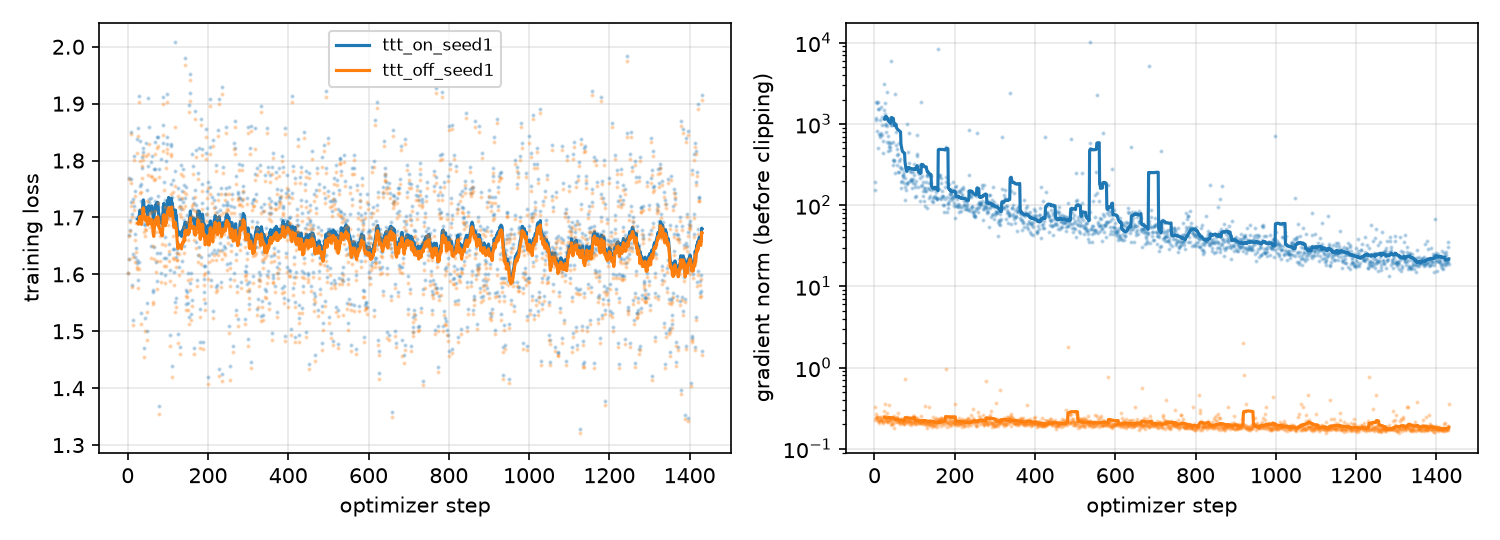
\includegraphics[width=\linewidth]{figures/curves_seed1.png}
\caption{Training loss (left) and pre-clipping gradient norm (right) per optimizer step for the seed-1 arms, which consume identical batches. Points are single steps and lines are running means. Seed 2 is in Appendix~\ref{app:figures}.}
\label{fig:curves}
\end{figure}

\begin{table}[H]
\caption{Same-batch training loss and pre-clipping gradient norm by phase of training (means over steps).}
\label{tab:phases}
\centering
\footnotesize
\resizebox{\textwidth}{!}{\begin{tabular}{lrrrrrr}
\toprule
Steps & Tokens & Loss TTT s1 / s2 & Loss control s1 / s2 & Gap s1 / s2 & Grad norm TTT s1 / s2 & Grad norm control \\
\midrule
1--150 & 0--0.31B & 1.701 / 1.702 & 1.684 / 1.682 & +0.017 / +0.020 & 546 / 578 & 0.23 \\
151--477 & 0.31--1.0B & 1.677 / 1.672 & 1.665 / 1.661 & +0.012 / +0.011 & 138 / 119 & 0.22 \\
478--954 & 1.0--2.0B & 1.656 / 1.658 & 1.647 / 1.649 & +0.009 / +0.009 & 93 / 68 & 0.21 \\
955--1288 & 2.0--2.7B & 1.648 / 1.660 & 1.641 / 1.653 & +0.008 / +0.008 & 30 / 32 & 0.20 \\
1289--1431 & 2.7--3.0B & 1.643 / 1.638 & 1.635 / 1.631 & +0.007 / +0.008 & 22 / 32 & 0.19 \\
\bottomrule
\end{tabular}}
\end{table}

\begin{table}[H]
\caption{Gradient norm by parameter group on two held-out 16k sequences (final checkpoints; the base model with a freshly initialised module as reference, two repeats).}
\centering
\footnotesize
\resizebox{\textwidth}{!}{\begin{tabular}{lrrrrr}
\toprule
Model & \texttt{ttt\_conv} (76.8k) & \texttt{ttt\_proj} (39.3M) & down-proj, TTT layers (149M) & other (3.87B) & total \\
\midrule
TTT, seed 1 & 49.58 & 0.42 & 0.31 & 0.95 & 49.60 \\
TTT, seed 2 & 49.15 & 0.42 & 0.31 & 0.94 & 49.16 \\
Control, seed 1 & -- & -- & -- & 0.99 & 0.99 \\
Control, seed 2 & -- & -- & -- & 0.97 & 0.97 \\
Base + fresh module & 17.0 / 18.1 & 0.00 & 0.36 & 1.24 & 17.1 / 18.2 \\
\bottomrule
\end{tabular}}
\end{table}

\begin{table}[H]
\caption{Held-out loss (eight 16k sequences, update active for the TTT arm) and inference cost (prefill of one held-out sequence plus 64 greedy tokens at batch size 1 on one GPU, best of three).}
\centering
\footnotesize
\begin{tabular}{lrr}
\toprule
 & Seed 1 & Seed 2 \\
\midrule
Held-out loss, base & 1.865 & 1.865 \\
Held-out loss, control & 1.823 & 1.822 \\
Held-out loss, TTT & 1.832 & 1.831 \\
\midrule
Seconds at 32k, TTT / control & 3.86 / 3.78 & 3.75 / 3.67 \\
Seconds at 64k, TTT / control & 7.31 / 7.28 & 7.24 / 7.09 \\
Peak GB at 32k, TTT / control & 15.95 / 15.57 & 15.95 / 15.57 \\
Peak GB at 64k, TTT / control & 23.38 / 23.00 & 23.38 / 23.00 \\
\bottomrule
\end{tabular}
\end{table}

\begin{table}[H]
\caption{Accumulated fast-weight change $\|W - W_0\|_F$ per TTT layer on eight held-out 32k sequences, after the first and after the seventh update, seeds 1 / 2. $\|W_0\|_F$ is 112 to 126.}
\centering
\footnotesize
\begin{tabular}{lrrr}
\toprule
Layer & after chunk 1 & after chunk 7 & relative to $W_0$ after chunk 7 \\
\midrule
0 & 0.13 / 0.10 & 0.76 / 0.62 & 0.64\% / 0.52\% \\
6 & 0.26 / 0.22 & 0.82 / 0.74 & 0.74\% / 0.67\% \\
12 & 0.10 / 0.11 & 0.49 / 0.54 & 0.42\% / 0.47\% \\
18 & 0.16 / 0.16 & 0.86 / 0.83 & 0.75\% / 0.73\% \\
24 & 0.21 / 0.18 & 1.01 / 0.93 & 0.86\% / 0.79\% \\
30 & 0.85 / 0.72 & 3.02 / 2.84 & 2.41\% / 2.26\% \\
\bottomrule
\end{tabular}
\end{table}

\section{Additional figures}\label{app:figures}

\begin{figure}[H]
\centering
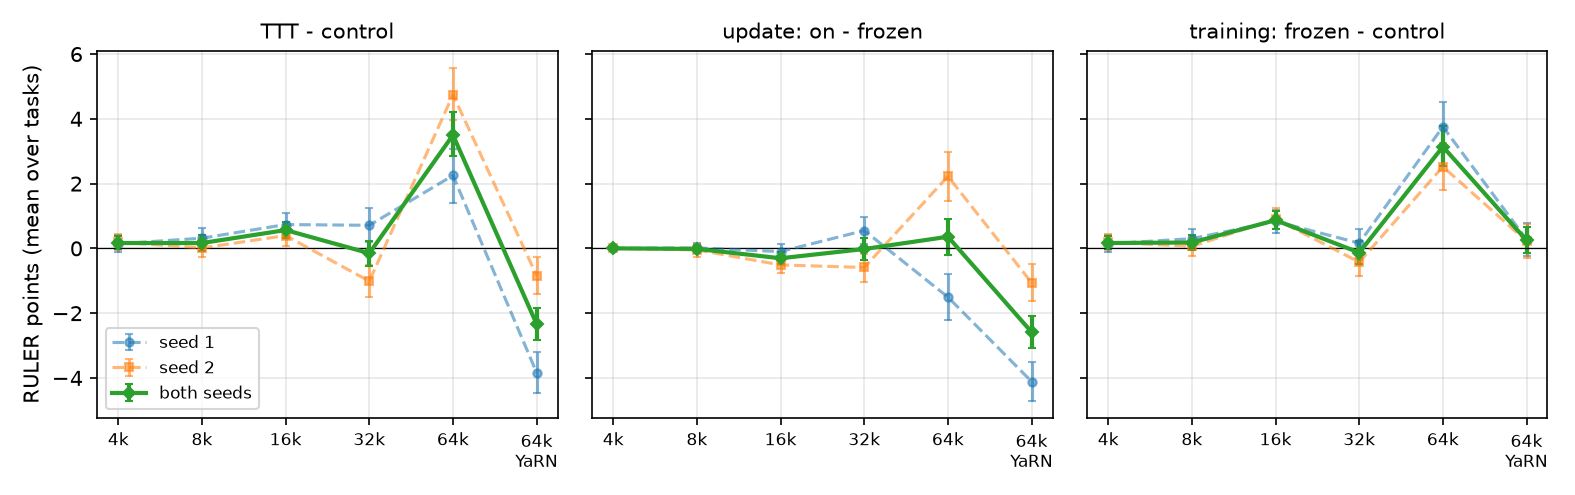
\includegraphics[width=\linewidth]{figures/effects_11.png}
\caption{The decomposition of Figure~\ref{fig:effects} on the 11 clean tasks.}
\end{figure}

\begin{figure}[H]
\centering
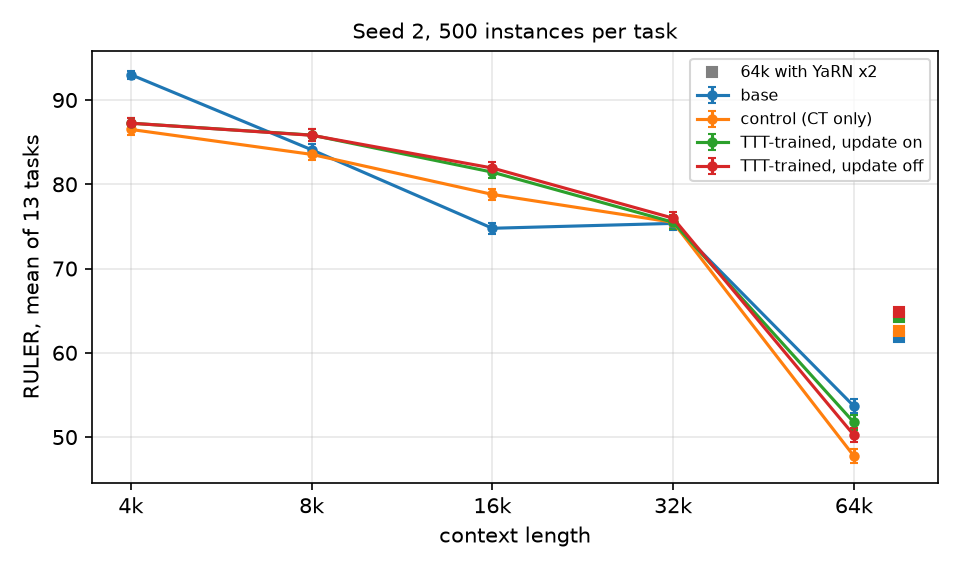
\includegraphics[width=0.78\linewidth]{figures/ruler_seed2.png}
\caption{RULER mean by context length for seed 2 (companion to Figure~\ref{fig:ruler}).}
\end{figure}

\begin{figure}[H]
\centering
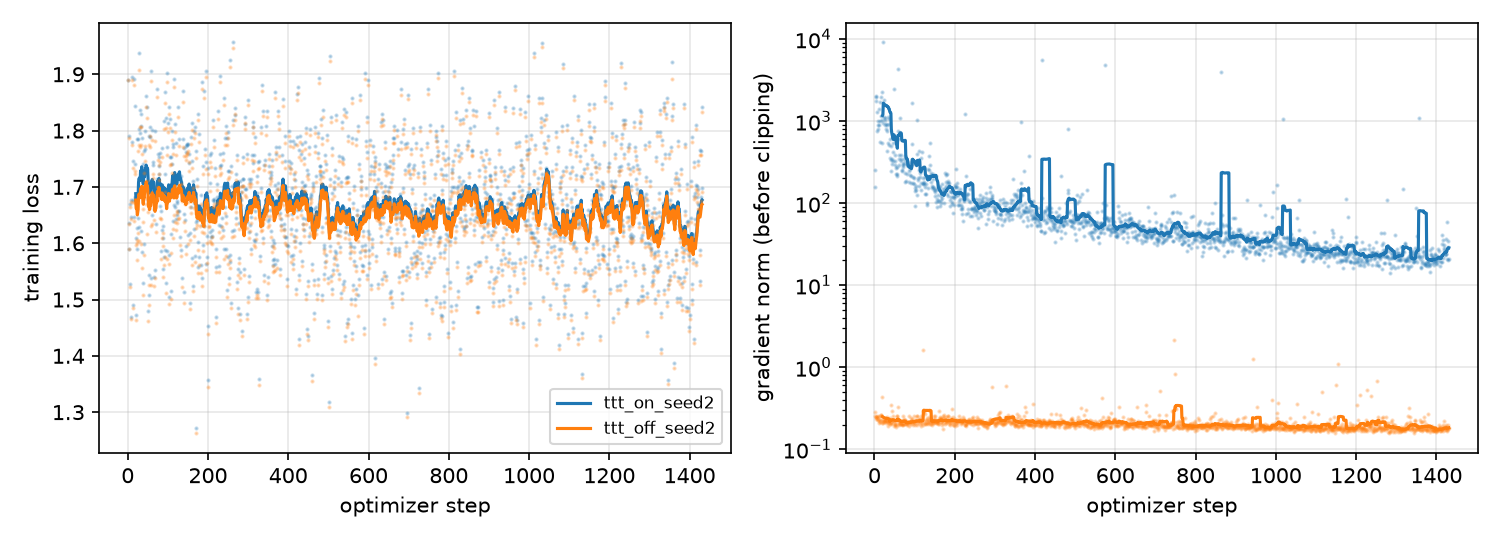
\includegraphics[width=\linewidth]{figures/curves_seed2.png}
\caption{Training loss and pre-clipping gradient norm for the seed-2 arms (companion to Figure~\ref{fig:curves}).}
\end{figure}

\end{document}
